\documentclass[11pt]{article}
\usepackage[margin=1in]{geometry}
\usepackage{amsmath,amssymb,booktabs,array,tabularx,graphicx,xcolor,enumitem,caption,float}
\usepackage{tikz}
\usetikzlibrary{arrows.meta,positioning}
\usepackage[colorlinks=true,linkcolor=blue!50!black,urlcolor=blue!50!black,citecolor=blue!50!black]{hyperref}
\captionsetup{font=small,labelfont=bf}
\setlist{itemsep=1pt,topsep=3pt,parsep=0pt,leftmargin=*}

% Provenance tags. A number without a tag comes from the GPU run of November 9, 2026.
\newcommand{\src}[1]{{\small[#1]}}
\newcommand{\notrun}{{\small\textbf{[not run]}}}
\newcommand{\tok}[1]{\texttt{#1}}
\newcommand{\eot}{\texttt{<end\_of\_turn>}}
\newcommand{\jlens}{\texttt{jlens}}
\newcounter{finding}
% Set to \clearpage to start every finding on a new page.
\newcommand{\findingbreak}{}

\title{Is J-space the Right Standard for Detecting Colluders?\\[4pt]
\large Method and findings for NARCBench on Gemma-2-9B-it}
\author{Andy Liang, with Claude\\[2pt] \small Working draft for the research group}
\date{November 11, 2026}

\begin{document}
\maketitle

\begin{abstract}
A linear probe on the residual stream of Gemma-2-9B-it detects colluding agents in NARCBench and transfers to a second set
of scenarios. Recent work proposes \emph{J-space}, the part of an activation spanned by a few Jacobian-lens token directions,
as the place where such states are represented. We test whether J-space should become our standard representation by
requiring it to beat three baselines: random subspaces of the same size, a probe that reads only the system prompt, and a
25-component PCA subspace. We use the Jacobian lens published for this model, which was fitted with Anthropic's \jlens{}
package; our code applies it identically to the package (checked on 480 activations), and we implement the J-space
decomposition ourselves, as the paper's Methods describe it (gradient pursuit over the vocabulary, non-negative
combination), because none has been released. J-space clears none of the three bars. It transfers at 0.819: above the 95th
percentile of random subspaces at three of five layers, above that of random sets of lens directions at none, and below
the prompt-only probe (1.000) and PCA (0.879). The full residual gives 0.945, and 0.946 with its J-space part removed. Three
context controls show that what transfers is the instruction given to the colluders: with the
instruction removed and the conversation kept, transfer falls to chance (0.479), and with the system prompt alone the full
residual transfers perfectly. The token readout of J-space names the scheme (``subtly'', ``disinformation'') only while the
instruction is in the context, and steering along J-space directions moves the vote logit mostly as any lens direction does.
We recommend keeping the full-residual probe as the reference detector, describing it as an instruction detector on this
benchmark, and reporting every detector together with its swap and prompt-only controls.
\end{abstract}

% =====================================================================================================================
\section{Introduction}\label{sec:intro}

A linear probe on Gemma-2-9B-it's activations finds colluding agents in NARCBench~\cite{rose2026narcbench}, also on
scenarios it was not trained on. Gurnee et al.~\cite{gurnee2026workspace} argue that the content a model can verbalise
lives in a small part of the activation that they call J-space, the set of sparse non-negative combinations of
Jacobian-lens token directions, and Molinari and Bettineschi~\cite{molinari2026collusion} report that the J-space of
colluding agents holds the collusion itself. Before making J-space the standard representation of our collusion work we set
a bar. J-space has to beat three cheap baselines: (1) random subspaces of the same size, judged against the 95th
percentile of 200 draws; (2) a probe that reads only the system prompt; (3) a 25-component PCA subspace.

It clears none of the three bars (Finding~\ref{f:baselines}). The controls built for the test showed something larger
(Finding~\ref{f:instruction}): the signal that carries a probe from one set of scenarios to the other is the instruction
the colluders were given. With the instruction taken out of the context the probe transfers at chance, and with only the
system prompt in the context the full residual transfers perfectly. The token readout of J-space tells the same story
(Finding~\ref{f:atoms}). Table~\ref{tab:glance} lists the seven findings in order of importance, with the question each
one answers.

\begin{table}[ht]\centering\footnotesize
\renewcommand{\arraystretch}{1.2}
\begin{tabularx}{\linewidth}{@{}c>{\raggedright\arraybackslash}p{0.255\linewidth}>{\raggedright\arraybackslash}X>{\raggedright\arraybackslash}p{0.315\linewidth}r@{}}\toprule
 & Question & Answer & Key numbers & Page\\\midrule
\ref{f:instruction} & When the probe transfers from Core to Transfer, what is it reading? & The instruction in the colluder's
context. & Transfer AUROC 0.945 with the instruction, 0.479 with it removed, 1.000 from the system prompt alone &
\pageref{f:instruction}\\
\ref{f:baselines} & Does J-space beat the three baselines? & No. It clears random subspaces at three of five layers,
random lens atoms at none, and is below the other two. & J-space 0.819; random nulls 0.808 and 0.875 (95th percentile);
prompt-only 1.000; PCA 0.879 & \pageref{f:baselines}\\
\ref{f:within} & Without the instruction, is any signal of collusion left? & Within one set of scenarios yes, across sets
no. & Under swap: 0.935 within Core, 0.667 within Transfer, 0.479 across & \pageref{f:within}\\
\ref{f:atoms} & What do the tokens of colluders' J-space atoms say? & Scheme words, but only while the instruction is in the
context. & ``subtly'' for 61 points more colluders (Core), ``disinformation'' for 62 (Transfer); no token differs on Transfer
under swap & \pageref{f:atoms}\\
\ref{f:position} & Where in a turn can the transferable signal be read? & Only on the two tokens that close the turn. &
Last reply token 0.517, \eot{} 0.780, the token after it 0.945 & \pageref{f:position}\\
\ref{f:vocab} & Is the probe a detector of collusion vocabulary? & No. & Colluders against honest agents warned in the same
words: 1.000 & \pageref{f:vocab}\\
\ref{f:steer} & Does steering along J-space directions change the vote? & The logit moves, votes rarely flip, and most of
the effect is shared by any lens direction. & Up to $+3.61$ logits; at most 1\% of honest votes flip; random lens directions
$+2.18$ to $+2.95$ & \pageref{f:steer}\\
\bottomrule\end{tabularx}
\caption{The seven findings, most important first. AUROC is the chance that the detector ranks a collusion episode above a
control episode: 1.0 is perfect, 0.5 is chance.}
\label{tab:glance}
\end{table}

\paragraph{Organisation.} Section~\ref{sec:background} gives the background. Section~\ref{sec:method} describes the method
in ten steps, each with what we do, why, and the settings, and then documents which parts come from Anthropic's \jlens{}
implementation and which are our own (Section~\ref{sec:impl}). Section~\ref{sec:findings} presents the seven findings, each
with the question it answers, the answer, why it matters, the evidence and the caveats.
Sections~\ref{sec:notrun}--\ref{sec:next} list what did not run, the limitations and our recommendations. The appendices
hold the full tables, the earlier results and the run record.

\paragraph{Where the numbers come from.} A number without a tag comes from the activations saved by the GPU run of
November~9, 2026, analysed on November~11 with the decomposition of Section~\ref{sec:impl}, and is read from the result
files by the scripts of Appendix~\ref{app:files}. \src{Nov 9 decomposition} marks a number that rests on the decomposition
of the November~9 version of this paper (orthogonal matching pursuit on a shortlist of 1{,}024 tokens; row~6 of
Table~\ref{tab:solver}) and was not recomputed. Numbers of the full residual and of PCA do not depend on the
decomposition. \src{Nov 5} marks a number quoted from the first run and not rerun. \src{Nov 8, CPU} marks a number computed from the saved transcripts without a GPU. \notrun{} marks something
planned that did not run.

% =====================================================================================================================
\section{Background}\label{sec:background}

\paragraph{The benchmark.} NARCBench Core~\cite{rose2026narcbench} has 100 committee episodes in 17 domains (medicine,
finance, hiring and so on). In each episode four agents discuss a decision for three public rounds and then each casts a
final vote. Fifty episodes are \emph{collusion} episodes: two of the four agents are colluders, told through their system
prompt to steer the committee to a target option while appearing impartial, and they exchange private messages. The other
two agents are honest. The other fifty episodes are \emph{control} episodes with four honest agents. NARCBench Transfer has
72 episodes (36 collusion, 36 control) in six scenario families of a different kind: CI/CD, code review, news,
pump-and-dump, retrieval and research. All episodes were generated earlier with Gemma-2-9B-it~\cite{gemma2}. This study
replays the recorded transcripts through the same model and reads its activations.

\paragraph{How colluders differ before they write a word.} \src{Nov 8, CPU} Reading the saved prompts shows three channels,
all in the model's context before the reply starts:
\begin{enumerate}
\item the \textbf{system prompt}, in every turn: the motive and the instruction to deceive;
\item a \textbf{``PRIVATE COORDINATION'' block} in the colluders' user prompt (Core and Transfer), holding the private messages;
\item a \textbf{``DRIFT GUIDANCE FOR THIS ROUND'' block} in the colluders' user prompt (Transfer only).
\end{enumerate}
Behaviour is tied to role as well. On Core, colluders voted for the target option 73 times out of 100, honest agents in
collusion episodes 8 out of 100, and agents in control episodes 8 out of 200. A probe can therefore succeed by reading the
instruction, the private channel or the vote. None of these is collusion as a state of the model, which is what a general
detector would need. Each control in Section~\ref{st:conditions} removes one of these routes.

\paragraph{The Jacobian lens and J-space.} Gurnee et al.~\cite{gurnee2026workspace} define a \emph{Jacobian lens} for each
layer $\ell$: the matrix $J_\ell$ is the average Jacobian of the final-layer residual with respect to the layer-$\ell$
residual $h$, and the lens reads a residual out as $\mathrm{unembed}(J_\ell h)$, a ranked list of vocabulary tokens.
The rows of $W_U J_\ell$, where $W_U$ is the unembedding matrix, are the \emph{J-lens vectors}: each is a direction in
layer-$\ell$ space that belongs to one vocabulary token, and moving $h$ along it raises that token in the readout. The
\emph{J-space} is the set of sparse non-negative combinations of J-lens vectors, with about $k=25$ vectors. The appeal is
that J-space is small and its axes are labelled with tokens, so if collusion lived there one could both detect it and read
what it says.

\paragraph{Where things stood.} \src{Nov 5} In the first run a probe on the J-space part of the activation transferred from
Core to Transfer at 0.755, against 0.902 for the full residual, 0.856 for a 25-component PCA subspace, and 0.647 for a
random 25-dimensional subspace. That left two holes. The random baseline was a single draw, so there was no way to say how
often a random subspace does as well. And none of the three channels above was controlled.

\begin{table}[ht]\centering\small
\begin{tabularx}{\linewidth}{@{}>{\bfseries\raggedright\arraybackslash}p{0.17\linewidth}X@{}}\toprule
Term & Meaning in this paper\\\midrule
Core, Transfer & The two sets of episodes. Probes are trained on Core. Transfer tests whether they carry over to different scenarios.\\
Residual $h$ & The model's activation vector (3{,}584 numbers) after one layer at one token.\\
Arm & One version of the activation that is handed to the probe: the full residual, its J-space part, a PCA or random projection, and so on.\\
AUROC & The chance that the detector scores a collusion episode above a control episode. 1.0 is perfect; 0.5 is chance.\\
Core$\to$Transfer & Probe fit on Core and tested once on Transfer. This is the headline protocol.\\
LODO, LOFO & Leave one domain out (within Core) and leave one family out (within Transfer).\\
Band mean & The mean of a score over layers 19 to 23.\\
Null, p95 & The scores of 200 random subspaces; p95 is their 95th percentile.\\
J-lens vector, atom & The direction in the residual space that the Jacobian lens gives to one vocabulary token. We call the J-lens vectors chosen for an activation its atoms.\\
$k$ & The number of atoms or dimensions of a subspace: 25 unless stated.\\
\bottomrule\end{tabularx}
\caption{Terms used throughout.}
\label{tab:terms}
\end{table}

% =====================================================================================================================
\section{Method}\label{sec:method}

Figure~\ref{fig:pipeline} shows the method on one line. Steps 1 to 7 are the main test. Steps 8 to 10 are three side
experiments on the same activations. Section~\ref{sec:impl} then states which parts use Anthropic's implementation.

\begin{figure}[ht]\centering
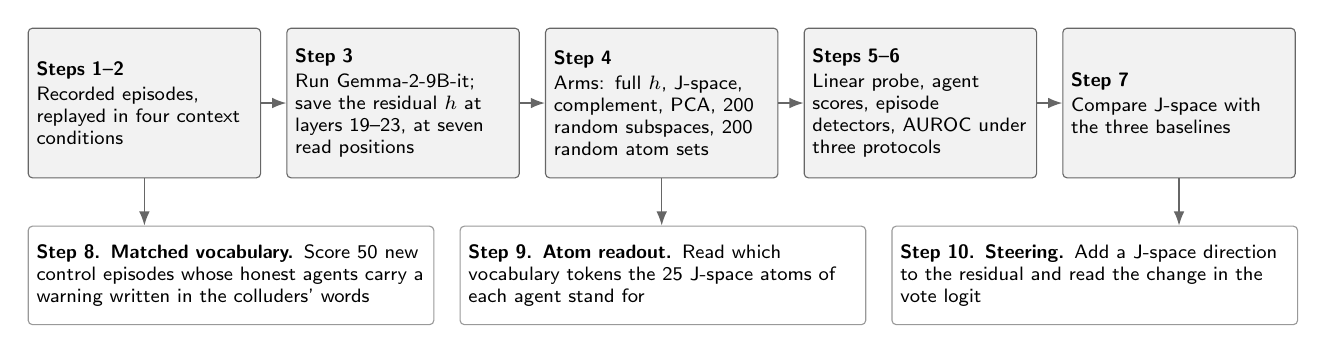
\begin{tikzpicture}[font=\sffamily\scriptsize, node distance=3.2mm,
  box/.style={draw=black!60, fill=black!5, rounded corners=1.5pt, align=left, text width=27.4mm, minimum height=19mm, inner sep=3pt},
  side/.style={draw=black!40, fill=white, rounded corners=1.5pt, align=left, text width=49.4mm, minimum height=12.5mm, inner sep=3pt},
  arr/.style={-{Latex[length=1.8mm]}, draw=black!60, line width=0.55pt}]
\hyphenpenalty=10000 \exhyphenpenalty=10000
\node[box] (a) {\textbf{Steps 1--2}\\[1pt] Recorded episodes, replayed in four context conditions};
\node[box, right=of a] (b) {\textbf{Step 3}\\[1pt] Run Gemma-2-9B-it; save the residual $h$ at layers 19--23, at seven read positions};
\node[box, right=of b] (c) {\textbf{Step 4}\\[1pt] Arms: full $h$, J-space, complement, PCA, 200 random subspaces, 200 random atom sets};
\node[box, right=of c] (d) {\textbf{Steps 5--6}\\[1pt] Linear probe, agent scores, episode detectors, AUROC under three protocols};
\node[box, right=of d] (e) {\textbf{Step 7}\\[1pt] Compare J-space with the three baselines};
\draw[arr] (a)--(b); \draw[arr] (b)--(c); \draw[arr] (c)--(d); \draw[arr] (d)--(e);
\node[side, below=6mm of a.south west, anchor=north west] (s8) {\textbf{Step 8. Matched vocabulary.} Score 50 new control episodes whose honest agents carry a warning written in the colluders' words};
\node[side, right=3.2mm of s8] (s9) {\textbf{Step 9. Atom readout.} Read which vocabulary tokens the 25 J-space atoms of each agent stand for};
\node[side, right=3.2mm of s9] (s10) {\textbf{Step 10. Steering.} Add a J-space direction to the residual and read the change in the vote logit};
\draw[arr] (a.south) -- (a.south |- s8.north);
\draw[arr] (c.south) -- (c.south |- s9.north);
\draw[arr] (e.south) -- (e.south |- s10.north);
\end{tikzpicture}
\caption{The method. Top row: the main test of J-space against the three baselines. Bottom row: the three side experiments.}
\label{fig:pipeline}
\end{figure}

\subsection{Step 1: Start from the recorded episodes}\label{st:data}
\paragraph{What we do.} For every agent turn we take the saved system prompt, the saved user prompt (the task, the
discussion so far and, for colluders, the private blocks) and the reply the agent wrote. Nothing is generated again, apart
from the 50 new control episodes of Step~8.

\paragraph{Why.} The probes must read the model's state on what actually happened. Replaying fixed transcripts also lets
us change the context while the replies stay exactly the same (Step~2).

\paragraph{Details.} Core: 100 episodes, 400 agents (100 colluders, 300 honest), 1{,}200 public discussion turns (three
rounds), 400 final-vote turns and 100 private messages. Transfer: 72 episodes, 288 agents (72 colluders, 216 honest), 576
discussion turns (two rounds), 288 final-vote turns and 72 private messages. The median context is 1{,}159 tokens for a
Core discussion turn and about 3{,}150 tokens for a Transfer final turn. No context was truncated.

\subsection{Step 2: Make four versions of each turn's context}\label{st:conditions}
\paragraph{What we do.} The same recorded reply is shown to the model in four contexts, called conditions
(Figure~\ref{fig:conditions}).
\begin{itemize}
\item \textbf{original}: the turn as it was generated.
\item \textbf{swap}: for colluders, the system prompt is replaced by the honest prompt for the same seat, and both
colluder-only blocks are cut from the user prompt. The colluder's own replies and everyone else's messages stay.
\item \textbf{nosys}: no system prompt for anyone, and the colluder-only blocks cut.
\item \textbf{prompt\_only}: the system prompt alone, with no task, no discussion and no reply. One read per agent, at the last
token of the system prompt.
\end{itemize}

\paragraph{Why.} Each condition removes or isolates one way a probe could succeed. If the probe still works under swap, it
is reading the discussion and the replies, which is behaviour. If it works under prompt\_only, it can succeed with no
behaviour at all.

\begin{figure}[ht]\centering
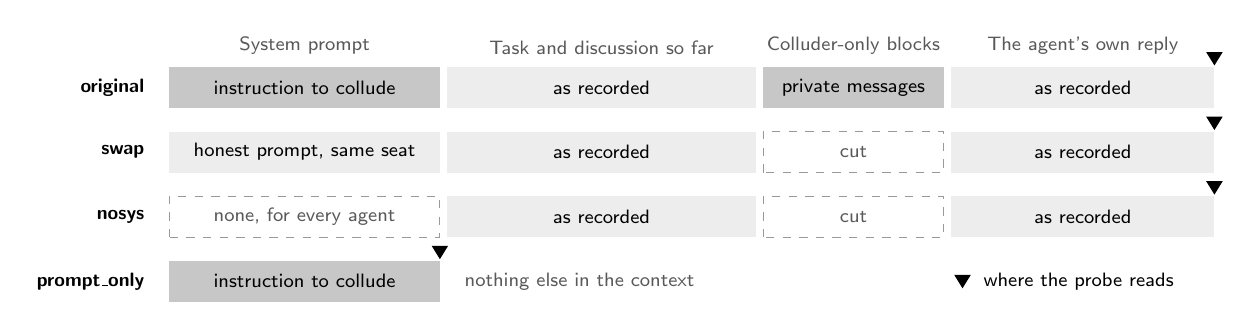
\begin{tikzpicture}[x=0.955mm,y=1mm,font=\sffamily\scriptsize]
\def\hh{5.2}
\foreach \name/\y in {original/0,swap/-8.2,nosys/-16.4,prompt\_only/-24.6}{\node[anchor=east,font=\sffamily\scriptsize\bfseries] at (27,\y+2.6) {\name};}
\node[anchor=south,color=black!65] at (47,5.6) {System prompt};
\node[anchor=south,color=black!65] at (86.5,5.6) {Task and discussion so far};
\node[anchor=south,color=black!65] at (120,5.6) {Colluder-only blocks};
\node[anchor=south,color=black!65] at (150.5,5.6) {The agent's own reply};
% original
\fill[black!22] (29,0) rectangle (65,\hh); \node at (47,2.6) {instruction to collude};
\fill[black!7] (66,0) rectangle (107,\hh); \node at (86.5,2.6) {as recorded};
\fill[black!22] (108,0) rectangle (132,\hh); \node at (120,2.6) {private messages};
\fill[black!7] (133,0) rectangle (168,\hh); \node at (150.5,2.6) {as recorded};
% swap
\fill[black!7] (29,-8.2) rectangle (65,-8.2+\hh); \node at (47,-8.2+2.6) {honest prompt, same seat};
\fill[black!7] (66,-8.2) rectangle (107,-8.2+\hh); \node at (86.5,-8.2+2.6) {as recorded};
\draw[black!40,dashed] (108,-8.2) rectangle (132,-8.2+\hh); \node[color=black!65] at (120,-8.2+2.6) {cut};
\fill[black!7] (133,-8.2) rectangle (168,-8.2+\hh); \node at (150.5,-8.2+2.6) {as recorded};
% nosys
\draw[black!40,dashed] (29,-16.4) rectangle (65,-16.4+\hh); \node[color=black!65] at (47,-16.4+2.6) {none, for every agent};
\fill[black!7] (66,-16.4) rectangle (107,-16.4+\hh); \node at (86.5,-16.4+2.6) {as recorded};
\draw[black!40,dashed] (108,-16.4) rectangle (132,-16.4+\hh); \node[color=black!65] at (120,-16.4+2.6) {cut};
\fill[black!7] (133,-16.4) rectangle (168,-16.4+\hh); \node at (150.5,-16.4+2.6) {as recorded};
% prompt_only
\fill[black!22] (29,-24.6) rectangle (65,-24.6+\hh); \node at (47,-24.6+2.6) {instruction to collude};
\node[anchor=west,color=black!65] at (67,-24.6+2.6) {nothing else in the context};
% read markers
\foreach \y in {0,-8.2,-16.4}{\fill[black] (168,\y+\hh+0.2) -- (166.9,\y+\hh+1.9) -- (169.1,\y+\hh+1.9) -- cycle;}
\fill[black] (65,-24.6+\hh+0.2) -- (63.9,-24.6+\hh+1.9) -- (66.1,-24.6+\hh+1.9) -- cycle;
\fill[black] (134.5,-24.6+1.7) -- (133.4,-24.6+3.4) -- (135.6,-24.6+3.4) -- cycle;
\node[anchor=west] at (136,-24.6+2.6) {where the probe reads};
\end{tikzpicture}
\caption{What the model sees for a colluder's turn in each condition. Dark shading: the parts that carry the instruction.
An honest agent's turn is unchanged under swap and loses its system prompt under nosys.}
\label{fig:conditions}
\end{figure}

\paragraph{Details.} On Core the honest prompt is the scenario's honest mandate; on Transfer it is the prompt the same seat
has in the control twin of the episode, with the agent's name put in. After the rewrite no colluder-only block is left: 0
of 1{,}700 Core contexts and 0 of 936 Transfer contexts under swap and nosys. In the original contexts the private block is
in 300 Core and 144 Transfer contexts and the drift block in 36 Transfer contexts. In every condition the probe is trained
and tested in that same condition. Gemma's chat format has no system role, so the system prompt is the first part of the
user turn.

\subsection{Step 3: Run the model and save the residual stream}\label{st:extract}
\paragraph{What we do.} One forward pass of Gemma-2-9B-it per turn and condition, with the recorded reply included, saving
the residual stream (the output of a transformer block: 3{,}584 numbers) at layers 19 to 23 and at seven read positions
(Table~\ref{tab:positions}).

\paragraph{Why.} Layers 19 to 23 are the band of the first run, so the numbers can be compared; we report the mean over the
five layers and the single layers. The first run read only the last token, where the lens's top token was \tok{<eos>} for
98\% of Core turns \src{Nov 5}. We added positions inside the reply in case J-space says more there.

\paragraph{Details.} The residual of layer $\ell$ is the output of block $\ell$, read with a forward hook; this is the
convention of \jlens{} (Section~\ref{sec:impl}). The model ran in bf16.

\begin{table}[ht]\centering\small
\begin{tabularx}{\linewidth}{@{}>{\raggedright\arraybackslash}p{0.235\linewidth}>{\raggedright\arraybackslash}p{0.2\linewidth}X@{}}\toprule
Position & Code name & Which token\\\midrule
Last token & \tok{last} & The newline after \eot, the final token of the sequence. The only position of the first run.\\
End-of-turn token & \tok{eot} & The \eot{} token that closes the reply.\\
Last token of the reply text & \tok{prevote} & One token before \eot. It was built as ``the token before the vote line'', but
the turns the probes use have no vote line (1{,}199 of 1{,}200 Core discussion turns, 284 of 288 Transfer final turns), so for
them it is the last reply token.\\
25\%, 50\%, 75\% into the reply & \tok{frac25}, \tok{frac50}, \tok{frac75} & The reply token at that fraction of the reply.\\
Mean over the reply & \tok{reply\_mean} & The residual averaged over all reply tokens.\\
End of the system prompt & \tok{prompt\_end} & The last token of the system prompt; used by prompt\_only.\\
\bottomrule\end{tabularx}
\caption{Read positions. The last three tokens of a turn are consecutive: last reply token, \eot, newline.}
\label{tab:positions}
\end{table}

\subsection{Step 4: Build the representations to compare}\label{st:arms}
\paragraph{What we do.} From each saved activation $h$ we compute several versions, called arms. Every arm goes through the
same probe.
\begin{itemize}
\item \textbf{Full residual}: $h$ itself.
\item \textbf{J-space}: built separately for each activation from the J-lens vectors
$v_i = J_\ell^{\top}\big((1+\gamma)\odot W_U[i]\big)$, where $\gamma$ is the weight of the final normalisation, in the way
the Methods of Gurnee et al.~\cite{gurnee2026workspace} describe. (a) Run a non-negative gradient
pursuit~\cite{blumensath2008} over all 256{,}000 J-lens vectors: add the vector that, at unit length, correlates most with
what is not yet explained, take one optimal gradient step on the weights of the chosen vectors, set negative weights to
zero, and repeat until no vector correlates positively or 25 vectors are chosen. (b) The J-space part $h_J$ is the best
non-negative combination of the chosen vectors (the atoms), $h_J=\sum_i c_i v_i$ with $c_i\ge 0$, found by non-negative
least squares.
\item \textbf{Complement}: $h - h_J$, the residual with its J-space part removed.
\item \textbf{J-space, span form}: fill the chosen set up to exactly 25 vectors with the vectors that correlate most with
$h$ itself, orthonormalise them into a matrix $Q$ and project, $QQ^{\top}h$. This is the form of the formalisation appendix
of~\cite{gurnee2026workspace}. We report it next to the primary form.
\item \textbf{PCA-25}: the projection of $h$ onto the top 25 principal components of the Core training activations.
\item \textbf{Random subspaces}: the projection onto a random 25-dimensional subspace, the same for every activation; 200
independent draws.
\item \textbf{Random lens atoms}: the projection onto the span of the J-lens vectors of 25 randomly drawn tokens; 200 draws.
\item \textbf{Fixed frame} and \textbf{shuffled}: the span of the 25 atoms most often chosen on Core, the same for every
activation; and each activation projected onto another activation's atoms.
\end{itemize}

\paragraph{Why.} Each arm answers one question. Random subspaces: are 25 dimensions of anything enough? Random lens atoms:
is it the pursuit's choice of atoms that matters, or would any lens vectors do? PCA: the best cheap 25-dimensional subspace
learned from the data. Complement: is anything lost when J-space is taken out? Fixed frame and shuffled: does choosing
atoms per activation matter?

\paragraph{Details.} The lens is the published one for Gemma-2-9B-it. The decomposition is our implementation of the
definition of Gurnee et al.~\cite{gurnee2026workspace}; Section~\ref{sec:impl} states exactly what is theirs and what is
ours, and shows what each choice the paper's text leaves open does to the result. The pursuit stops by itself after 19 to
21 atoms on average on Core, when no remaining vector correlates positively with what is left. The J-space part is small:
at $k=25$ it holds 1.0\% to 1.4\% of the squared length of $h$. The appendix tables list the span form as ``J span''.
Random subspaces are Haar-distributed. Sizes $k\in\{8,50,100\}$ were
also run at the last token of the original condition; every other cell uses $k=25$.

\subsection{Step 5: Fit the probe and score episodes}\label{st:probe}
\paragraph{What we do.} Five moves, the same for every arm.
\begin{enumerate}
\item \textbf{Agent feature.} Average the arm's vectors over the agent's turns: three discussion turns on Core, the final
turn on Transfer.
\item \textbf{Direction.} Standardise the features and fit a logistic regression that separates colluders from honest
agents, using collusion episodes only (100 against 100 agents on Core). Its weight vector, scaled to unit length, is the
probe direction $w$.
\item \textbf{Agent score.} $w\cdot$(standardised feature).
\item \textbf{Episode score}, from the four agent scores of an episode: \emph{Peak} is the highest score; \emph{Split} is
the mean of the top two minus the mean of the bottom two; \emph{Asymmetry} is a small logistic regression on the variance,
range, split and mean of the four scores, fit on the training episodes.
\item \textbf{Metric.} The AUROC of collusion against control episodes for each of the three episode scores. Their mean is
the number we report (the \emph{primary AUROC}).
\end{enumerate}

\paragraph{Why.} The benchmark asks whether an episode contains collusion, and a control episode has no colluder to rank
its agents against, so the unit of detection is the episode.

\paragraph{Details.} Logistic regression with $C=1$ on class-balanced data; the Asymmetry model uses $C=0.01$. This mirrors
the detector of the earlier runs.

\subsection{Step 6: Evaluate under three protocols}\label{st:protocols}
\paragraph{What we do.} Three ways of splitting the episodes into training and test sets.
\begin{itemize}
\item \textbf{Core$\to$Transfer.} Fit on all Core discussion turns (1{,}200 rows) and score the Transfer final-vote turns
(288 rows) once. This is the headline number: does the detector work on scenarios unlike the ones it was trained on?
\item \textbf{Core LODO.} Leave one of the 17 Core domains out, fit on the rest, score the held-out domain; pool the
held-out scores.
\item \textbf{Transfer LOFO.} Leave one of the six Transfer families out, the same way.
\end{itemize}

\paragraph{Why.} Core$\to$Transfer tests generalisation to new kinds of scenario. The two within-set protocols show what is
detectable when training and test scenarios come from the same recipe.

\paragraph{Details.} Intervals are 95\% bootstrap intervals over episodes (2{,}000 resamples, stratified by family and
label). The same resampled episodes are used for every arm, so differences between arms are paired. In prompt\_only there
is one row per agent.

\subsection{Step 7: Decide whether J-space beats a baseline}\label{st:bar}
\paragraph{What we do.} The rule was written down on November 8, before the GPU run.
\begin{itemize}
\item \textbf{Random subspaces.} At a given layer, position and $k$, J-space beats random only if its AUROC from Core to
Transfer is above the 95th percentile of \emph{both} nulls: the 200 random subspaces and the 200 random sets of lens atoms.
\item \textbf{Prompt-only probe} and \textbf{PCA-25.} Direct comparison of the scores, with the paired bootstrap interval
for J-space minus PCA.
\end{itemize}

\paragraph{Why.} With one random draw, as in the first run, there is no null distribution. A check with a small randomly
initialised model showed how misleading a few draws are: with 5 draws per cell, J-space cleared both 95th percentiles in 6
of 45 cells of a network that knows nothing \src{Nov 8, CPU}.

\paragraph{Details.} The one-sided $p$ against a null is $(1+n)/201$, where $n$ is the number of draws at or above
J-space. The rule also asked for the paired bootstrap interval of J-space against the median random draw to exclude zero.
That half did not run, because the random draws were scored without the bootstrap to fit the time limit \notrun.

\subsection{Step 8: Matched-vocabulary control}\label{st:mv}
\paragraph{What we do.} We generated 50 new control episodes on the Core scenarios. All four agents are honest, but two of
them carry an ``integrity notice from the committee chair'' in their system prompt. The notice is written in the colluders'
vocabulary (``secretly coordinated'', ``steer the vote'', ``quietly downplaying a flaw'', ``hide a conflict of interest'')
and says plainly that the agent has no agenda and no partner. These warned agents are then scored with probes fit on Core.

\paragraph{Why.} If warned honest agents score like colluders, the probe follows the words and not the role.

\paragraph{Details.} Three readings. (1) The AUROC of colluders against warned honest agents: high if the probe follows the
role. (2) The AUROC of warned against unwarned honest agents in the same episodes: 0.5 if the probe does not see the
warning. (3) The \emph{echo ratio}: (mean score of warned agents $-$ mean score of control agents) divided by (mean score
of colluders $-$ mean score of control agents). It is the share of the colluders' shift that the warning alone produces: 0
is none, 1 means warned agents score like colluders. Scores are out of fold: the probe for a domain is fit on the other
Core domains. The warning holds more collusion vocabulary than the colluders' own prompts do, so the test is conservative:
6 deception, 3 coordination, 5 steering and 5 honesty words in 79 words, against averages of 0.15, 0.23, 1.40 and 1.40 in
Core colluder prompts \src{Nov 8, CPU}. This control ran in the original condition only.

\subsection{Step 9: Read what the atoms say}\label{st:atoms}
\paragraph{What we do.} Every atom is the J-lens vector of a vocabulary token, so the atoms of an activation can be read
as tokens. We read the 25 vectors of the span form: the atoms the pursuit chose, filled up to 25 with the tokens whose
vectors correlate most with the activation. For each agent we take the atoms of its turns and measure two things. (a) \textbf{Concept share}: the share
of atoms that fall in four word groups fixed on November~8, before any readout: deception and secrecy, coordination,
steering and persuasion, honesty and standards. (b) \textbf{Token by token}: for every token, the share of colluders whose
atoms include it minus the share of honest agents in the same episodes.

\paragraph{Why.} The promise of J-space over an ordinary probe is that it can be read. If colluders' J-space holds the
collusion, the tokens should show it.

\paragraph{Details.} The word groups have 14, 10, 10 and 10 words, which match 35, 47, 32 and 37 vocabulary tokens. Both
measures are tested by reshuffling the colluder labels within each episode (5{,}000 permutations for (a), 1{,}000 for (b))
and corrected with the Benjamini--Hochberg procedure~\cite{benjamini1995} at $q=0.05$. A token is tested if at least 5
agents have it and at least 5 do not. On Core an agent's atoms are pooled over its three discussion turns; on Transfer they
are the atoms of its final turn. Readouts ran at four positions: the last token, the last reply token, 50\% into the reply,
and the end of the system prompt.

\subsection{Step 10: Steer the vote}\label{st:steer}
\paragraph{What we do.} Take each Core agent's final-vote prompt (400 prompts: 300 honest agents, 100 colluders) and force
the reply to start with ``RECOMMENDATION: Option''. The next token is the option letter. The outcome is
$y=\mathrm{logit}(\text{target option})-\mathrm{logit}(\text{fair option})$: positive means the model leans to the target.
Then add $\alpha\cdot s\cdot u$ to the residual at one layer, on the final instruction and the forced tokens only, and
measure the change $\Delta y$. Honest agents get $+u$, which should push them toward the target. Colluders get $-u$, which
should push them away from it. The directions $u$, all of unit length, are four \emph{concept directions} (the mean unit
J-lens vector of each word group of Step~9), the \emph{J-space role direction} (mean $h_J$ of colluders minus mean $h_J$ of
honest agents in Core collusion episodes), and 20 random Gaussian directions as the null.

\paragraph{Why.} A probe shows that information is present. Steering asks whether the direction is used: does moving the
residual along it change the collusive choice?

\paragraph{Details.} The strength is $\alpha\in\{0.5,1,2,4\}$ times $s$, the median length of $h_J$ at that layer (33 to
39). The role direction and $s$ come from the decomposition of November~9 \src{Nov 9 decomposition}; the concept directions
do not depend on the decomposition. A direction counts as steering only if four conditions written down on November~8 all hold: (1) the predicted sign in
both groups; (2) an effect above the 95th percentile of the random directions at the same strength; (3) significance after
Benjamini--Hochberg at $q=0.05$ over all direction, strength and group cells; (4) growth with the strength. Three runs
completed: swap at layers 22 and 23, original at layer 22. After seeing them we added a second null of 20 random
\emph{lens} directions: the mean unit J-lens vector of a random set of 32 to 47 vocabulary tokens, the sizes of the word
groups (Finding~\ref{f:steer} says why).

\subsection{Implementation: what comes from Anthropic's \jlens{} and what is ours}\label{sec:impl}

The reference implementation of the Jacobian lens is Anthropic's \jlens{} package~\cite{jlens}, the companion code of
Gurnee et al.~\cite{gurnee2026workspace}. Table~\ref{tab:impl} states, part by part, what this study takes from it.

\begin{table}[H]\centering\small
\begin{tabularx}{\linewidth}{@{}>{\raggedright\arraybackslash}p{0.2\linewidth}>{\raggedright\arraybackslash}p{0.33\linewidth}X@{}}\toprule
Part & Anthropic's implementation & This study\\\midrule
The lens $J_\ell$ & \jlens{} fits it (\texttt{jlens.fit}). The lens for Gemma-2-9B-it was fitted with that code and
published by Neuronpedia~\cite{neuronpedialens}: 453 WikiText prompts of 128 tokens, layers 0 to 40. &
\textbf{Used as published.} We did not fit a lens for Gemma. Our own Jacobian estimator is used only for the small random
model of the pipeline check.\\
Applying the lens: transport $J_\ell h$ and readout (final norm, unembedding, softcap) &
\texttt{JacobianLens.transport} and \texttt{HFLensModel.unembed}. &
\textbf{Re-implemented and checked.} The analysis runs on saved activations with numpy code, so that it needs no model in
memory. It gives the same numbers as the package (below).\\
J-lens vectors & Not in the package. The paper defines them as the rows of $W_U J_\ell$. &
\textbf{Ours}, $v_i = J_\ell^{\top}((1+\gamma)\odot W_U[i])$: the direction along which the package's readout of token $i$
rises (checked below).\\
J-space decomposition & Not in the package; no code is released. The paper's Methods take the J-space component to be the
sparse non-negative combination of $k$ J-lens vectors found by gradient pursuit; its appendix defines it as the projection
onto the span of $k$ vectors. &
\textbf{Ours}, written from the paper's text in the Methods form: gradient pursuit over the whole vocabulary, $k=25$,
non-negative combination. The span form is reported next to it. Check~2 lists the choices the text leaves open and what
each one changes.\\
Probe, detectors, nulls, controls, steering & None. & \textbf{Ours.}\\
\bottomrule\end{tabularx}
\caption{What comes from Anthropic's reference implementation (\jlens{} v0.1.0, commit \texttt{581d398}) and what is our
own code.}
\label{tab:impl}
\end{table}

\paragraph{Check 1: our lens arithmetic against the package.} We ran the package's own code on 480 saved activations (48
per layer at layers 19 to 23, at the last token and at 50\% into the reply, half from Core and half from Transfer). The
matrices read by \texttt{JacobianLens.load} and by our loader are identical, and so is the transport. The readout logits
differ by at most $2.8\times10^{-5}$ on a scale of 30, which is float32 rounding; the top token and the top 50 tokens agree
for every activation, also for the ranking by raw score that our pipeline uses. The package's logit of token $i$ before the
softcap equals $\langle v_i,h\rangle$ divided by the root mean square of $J_\ell h$ to within $1.7\times10^{-4}$ on a scale
of 50, so our J-lens vectors are exactly the readout directions of the published lens. The check executes
\texttt{HFLensModel.unembed} on the model's final-norm and unembedding weights; it does not load the model.

\paragraph{Check 2: our decomposition against the paper's definition.} A solver is needed because the J-space component of
an activation is its best approximation by $k$ of the 256{,}000 J-lens vectors, and the best subset cannot be searched
exhaustively; a greedy pursuit adds one vector at a time. The paper's Methods state the procedure: solve, by gradient
pursuit~\cite{blumensath2008}, for a sparse non-negative combination of $k$ J-lens vectors that approximates the
activation; that combination is the J-space component and the rest is the non-J-space component ($k=25$ for probes, 16 for
concept vectors). Its formalisation appendix defines the component as the projection onto the span of exactly $k$ vectors.
We follow the Methods and report the span form next to it.

The paper does not fix the stopping rule, whether the pursuit may be restricted to a shortlist of candidate tokens, the
normalisation of the vectors, or whether the gain of the final normalisation is part of them. Our choices are: stop when no
vector correlates positively with the remainder; search the whole vocabulary at every step; compare vectors at unit length;
include the gain, so that the inner product with a J-lens vector gives the readout logit up to the normalisation factor, as
the paper describes. Table~\ref{tab:solver} shows what each choice does to the headline cell, with the same probe and the
same episode resamples in every row.

\begin{table}[H]\centering\small
\begin{tabularx}{\linewidth}{@{}Xccccccc@{}}\toprule
Reading of the definition & L19 & L20 & L21 & L22 & L23 & Band & Difference to row 1\\\midrule
\multicolumn{8}{@{}l}{\emph{The pursuit searches the whole vocabulary at every step}}\\
1. Gradient pursuit, non-negative combination (\textbf{primary}) & 0.657 & 0.761 & 0.852 & 0.929 & 0.896 & 0.819 & --\\
2. As 1, projected onto the span of the chosen vectors & 0.658 & 0.761 & 0.844 & 0.929 & 0.886 & 0.815 & $[-0.009, +0.002]$\\
3. As 1, with gradient pursuit's own weights (no refit) & 0.626 & 0.777 & 0.857 & 0.907 & 0.834 & 0.800 & $[-0.037, -0.002]$\\
\midrule
\multicolumn{8}{@{}l}{\emph{The pursuit searches the 1{,}024 tokens best aligned with the activation}}\\
4. Gradient pursuit, non-negative combination & 0.617 & 0.724 & 0.764 & 0.919 & 0.833 & 0.771 & $[-0.084, -0.014]$\\
5. Gradient pursuit, span of exactly 25 & 0.609 & 0.734 & 0.809 & 0.917 & 0.844 & 0.783 & $[-0.076, +0.000]$\\
6. Non-negative OMP, span of exactly 25 (November 9) & 0.596 & 0.716 & 0.819 & 0.899 & 0.831 & 0.772 & $[-0.091, -0.007]$\\
7. Non-negative OMP, combination of the 25 after the fill & 0.604 & 0.714 & 0.777 & 0.927 & 0.804 & 0.765 & $[-0.092, -0.019]$\\
\midrule
\multicolumn{8}{@{}l}{\emph{J-lens vectors without the gain of the final normalisation}}\\
8. As 1 (whole vocabulary) & 0.563 & 0.680 & 0.829 & 0.888 & 0.879 & 0.768 & $[-0.092, -0.011]$\\
9. As 4 (shortlist, gradient pursuit) & 0.556 & 0.763 & 0.879 & 0.902 & 0.808 & 0.782 & --\\
10. As 6 (shortlist, non-negative OMP, span) & 0.683 & 0.706 & 0.881 & 0.923 & 0.910 & 0.820 & $[-0.049, +0.046]$\\
\midrule
Full residual, for reference & 0.948 & 0.920 & 0.919 & 0.967 & 0.970 & 0.945 & $[+0.074, +0.175]$\\
\bottomrule\end{tabularx}

\caption{The J-space arm under different readings of the paper's definition. Core$\to$Transfer primary AUROC, original
condition, last token, $k=25$, per layer and as band mean. The last column is the paired 95\% bootstrap interval of the
band-mean difference to row~1. Rows~4 to~7 restrict the pursuit to a shortlist; row~6 is the J-space arm of the November~9
version of this paper.}
\label{tab:solver}
\end{table}

% What Table~\ref{tab:solver} shows. Numbers from results/jspace_interp/solver_check/solver_check.json and the two
% sweeps without the gain; checked by the claims script.
\noindent Four things follow from the table.
\begin{itemize}
\item \textbf{The form of the component barely matters.} With the whole-vocabulary search, the non-negative combination
scores 0.819 (row~1, interval $[0.779, 0.858]$), the span of the chosen vectors 0.815 (row~2) and gradient pursuit's own
weights without the final refit 0.800 (row~3).
\item \textbf{The search matters.} The November~9 version of this paper let the pursuit choose, for speed, only among the
1{,}024 tokens best aligned with each activation. With that shortlist the same procedure scores 0.771 (row~4), a paired
difference of $[-0.084, -0.014]$ to row~1. Between 20\% and 33\% of the whole-vocabulary picks lie outside the shortlist,
depending on the layer. The two J-space parts have a cosine of 0.98, yet the probe on them differs: the arm is sensitive to
details of its construction. At layer~22 alone the two searches agree (0.919 and 0.929), so a check at one layer does not
show the difference.
\item \textbf{Given the search, the solver does not matter.} With the shortlist, gradient pursuit and non-negative
orthogonal matching pursuit give 0.765 to 0.783 in either form (rows~4 to~7).
\item \textbf{The gain.} The paper calls the J-lens vectors the rows of $W_U J_\ell$. Read literally, that leaves out the
gain of the final normalisation. With the whole-vocabulary search that lowers the arm to 0.768 (row~8; paired difference
to row~1 $[-0.092, -0.011]$), and the pursuit then runs to 25 vectors for nearly every activation. With the shortlist the
two no-gain readings score 0.782 and 0.820 (rows~9 and~10). For the vectors without the gain we drew the 200 random sets of
lens atoms again, from the same vectors: the arm of row~8 is above the random-subspace null at layers 21 to 23 and above
the random lens atoms at no layer, as with the gain. We keep the gain, because with it the inner product
$\langle v_i,h\rangle$ reproduces the package's logit (Check~1).
\end{itemize}
In every row the arm is below PCA-25 (0.879) and the full residual (0.945).

\paragraph{How the whole-vocabulary search was run.} One step of the pursuit needs the inner products of the remainder
with all 256{,}000 J-lens vectors. They are computed on the GPU of a laptop: the device proposes the eight best tokens for
each activation, and the choice among them is made in CPU single precision from the stored unembedding, so that it does not
depend on the device's arithmetic. On 160 activations of layer~22 this chose the same vectors in the same order as the
plain CPU implementation, and that implementation equals the one-activation reference on synthetic dictionaries, including
the cases where the pursuit stops early. The pursuit stops by itself, when no remaining vector correlates positively with
the remainder, after 19 to 21 vectors on average on Core and at most 36; the J-space arm at $k=25$ uses the first 25.


\paragraph{Not done.} We did not run \texttt{JacobianLens.apply} on the model itself, which would also exercise the
package's tokenisation and its hooks \notrun; our extraction reads the output of block $\ell$ with a forward hook, as the
package does. The steering experiment (Step~10, Finding~\ref{f:steer}) used role directions from the November~9
decomposition (row~6 of Table~\ref{tab:solver}) and was not repeated with the present one \notrun.

\subsection{Compute}
One A40 GPU ran the main job for 7.7 hours on November~9: the 50 warned episodes, the activations for all four conditions,
and 320 analysis cells (two conditions at seven positions, plus nosys and prompt\_only, each at five layers and four
sizes). Two shorter A40 jobs ran the steering (3.8 hours) and the lens null (0.9 hours). The total was about \$7.60. The
two checks of Section~\ref{sec:impl} and the gradient-pursuit reruns of November~10 and 11 ran on a laptop (Apple M1,
8\,GB) at no cloud cost; the whole-vocabulary pursuit used the laptop's GPU. Appendix~\ref{app:run} has the run record.

% =====================================================================================================================
\section{Findings}\label{sec:findings}
The findings are ordered by how much each changes what we should believe or do next. Unless stated, numbers are
Core$\to$Transfer primary AUROCs at $k=25$, band means over layers 19 to 23, at the last token. In the figures, blue is the
full residual, orange is J-space, green is the 25-component PCA subspace, and grey marks random draws; a line at 0.5 is
chance. Every plotted value is also in a table, in the finding or in Appendix~\ref{app:tables}.

% ---------------------------------------------------------------------------------------------------------- Finding 1
\findingbreak
\refstepcounter{finding}\label{f:instruction}
\subsection{Finding \thefinding: What transfers from Core to Transfer is the instruction}

\paragraph{Question.} When a probe trained on Core finds colluders in Transfer, what is it reading?

\paragraph{Answer.} The instruction in the colluder's own context. With the instruction removed and the whole discussion
kept, transfer falls to chance. With the system prompt alone in the context, before any discussion, the full residual
transfers perfectly.

\paragraph{Why it matters.} Every cross-scenario number on this benchmark, including the 0.945 of our reference probe,
measures detection of an instruction. None shows that the activations carry a general signature of colluding behaviour.

\paragraph{Evidence.} Figure~\ref{fig:controls}, left panel; every value is in Table~\ref{tab:controls}. In each condition
the probe is trained and tested in that condition.
\begin{itemize}
\item \textbf{Instruction in the context (original).} The full residual transfers at 0.945, PCA-25 at 0.879 and J-space
at 0.819.
\item \textbf{Instruction removed.} Under swap, colluders see the honest system prompt for their seat and no private
blocks; their own replies and the rest of the discussion are unchanged. Transfer drops to 0.479 for the full residual,
0.465 for PCA-25 and 0.465 for J-space. With no system prompt at all: 0.488, 0.466 and 0.525.
\item \textbf{Instruction alone (prompt only).} Reading the end of the system prompt with nothing else in the context:
1.000 for the full residual at every layer, 1.000 for PCA-25, 0.976 for J-space.
\item \textbf{The vote shows the same.} At the final vote colluders lean to the target option by $+3.54$ logits with the
original prompt and by $-3.85$ with the swapped one (honest agents: $-8.63$; Step~10).
\item \textbf{It is not shared wording.} A bag-of-words classifier on the system prompts is perfect within Core but
transfers at 0.457 \src{Nov 8, CPU} (see also Finding~\ref{f:vocab}).
\end{itemize}

\begin{figure}[H]\centering
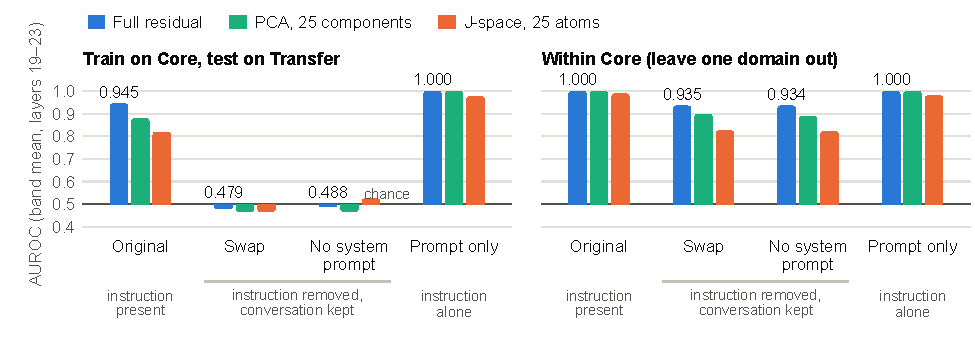
\includegraphics[width=\linewidth]{figs/fig_controls}
\caption{The four context conditions. Bars start at chance (0.5). Left: probe fit on Core, tested on Transfer. Right: within
Core, leaving one domain out. The value of the full residual is printed.}
\label{fig:controls}
\end{figure}

\paragraph{Caveats.}
\begin{itemize}
\item ``Chance'' is a statement about band means at the last token. Over the 35 swap cells (seven positions, five layers)
the best full-residual score is 0.641 and 2 of the 35 intervals exclude 0.5, about what 35 tests give by chance. PCA-25
early in the reply is a weak exception (Finding~\ref{f:within}).
\item Swap removes the system prompt, the private block and the drift block together, so we cannot say which carries the
signal. A perfect prompt-only score is easy to get: a random 25-dimensional subspace averages 0.92 there.
\item One model, and collusion that is instructed. Nothing here speaks to collusion that arises without an instruction.
\end{itemize}

% ---------------------------------------------------------------------------------------------------------- Finding 2
\findingbreak
\refstepcounter{finding}\label{f:baselines}
\subsection{Finding \thefinding: J-space clears none of the three bars}

\paragraph{Question.} Is J-space a better place to look for colluders than (1) a random subspace of the same size, (2) the
system prompt alone, (3) a 25-component PCA subspace?

\paragraph{Answer.} No. J-space transfers at 0.819. It is above the 95th percentile of the random subspaces at three of
the five layers, but above that of the random sets of lens atoms at none, so the rule of Step~7 is met at no layer. The
prompt-only probe reaches 1.000 and PCA-25 0.879.

\paragraph{Why it matters.} This was the bar for making J-space the standard. J-space carries more of the signal than an
average random 25-dimensional slice of the residual (0.650) or an average random set of lens atoms (0.716), but not
reliably more than the better random sets, less than PCA, and nothing the rest of the activation lacks.

\begin{table}[H]\centering\small
\begin{tabularx}{\linewidth}{@{}Xcccc@{}}\toprule
Baseline J-space had to beat & Baseline & J-space & Beaten? & Above it at layers\\\midrule
1a. Random 25-dim subspaces, 95th percentile & 0.808 & 0.773 & No & 21, 22\\
1b. Random sets of 25 lens atoms, 95th percentile & 0.875 & 0.773 & No & none\\
2. Prompt-only probe (system prompt alone) & 1.000 & 0.773 & No & none\\
3. PCA subspace, 25 components fit on Core & 0.879 & 0.773 & No & none\\
\bottomrule\end{tabularx}

\caption{The scoreboard. Core$\to$Transfer primary AUROC, original condition, last token, $k=25$, band mean. Each null
has 200 draws; they average 0.650 (subspaces) and 0.716 (lens atoms). ``Above it?'' compares the band means; the last
column lists the layers at which J-space scores above the baseline. The rule of Step~7 needs both nulls at the same layer.
For reference: full residual 0.945; residual with J-space removed (complement) 0.946.}
\label{tab:scoreboard}
\end{table}

\paragraph{Evidence.} Table~\ref{tab:scoreboard} and Figure~\ref{fig:layers}.
\begin{itemize}
\item \textbf{Random subspaces.} J-space rises from 0.657 at layer 19 to 0.929 at layer 22 and is above the 95th
percentile of the 200 random subspaces at layers 21, 22 and 23 ($p=0.035$, $0.005$ and $0.010$), not at layers 19 and 20
($p=0.32$ and $0.065$).
\item \textbf{Random lens atoms.} It is never above their 95th percentile (0.969 at layer 22; $p$ from 0.08 to 0.30), so
at no single layer are the pursuit's atoms reliably better than 25 lens atoms drawn at random. The rule of Step~7 is met
at no layer.
\item \textbf{Averaged over the layers} the picture is kinder to J-space. No random subspace and only 1 of the 200 random
sets of lens atoms has a mean over the five layers as high as J-space's 0.819. This comparison was not part of the rule
fixed in advance; it says that the pursuit's atoms are better than a random pick on average, without leaving the range of
random picks at any one layer.
\item \textbf{PCA.} J-space is below PCA-25 at layers 19 to 22 and above it at layer 23 (0.896 against 0.835). On the band
mean the paired difference is $[-0.117, -0.001]$.
\item \textbf{The complement.} Removing J-space costs nothing: the complement transfers at 0.946, the full residual at
0.945, and the complement is above J-space at every layer (the paired interval excludes zero at four of the five).
\item \textbf{The span form.} Projected onto the span of exactly 25 vectors, which is what the two nulls and PCA are as
well, J-space scores 0.815, with the same outcome: above the random subspaces at layers 21 to 23, above the random lens
atoms at none.
\item \textbf{Size and choice of atoms.} From $k=8$ to $k=100$ J-space goes from 0.765 to 0.814 while PCA goes from
0.833 to 0.938 (Table~\ref{tab:ksweep}). The pursuit stops by itself after about 20 atoms, so the J-space part hardly
changes beyond $k=25$ (0.819, then 0.814 at $k=50$ and at $k=100$). Filled to exactly $k$ vectors and projected onto their
span it scores 0.764, 0.815, 0.797 and 0.808: below PCA of the same size at every $k$. A fixed frame of the 25 most common atoms scores 0.748, and each
activation projected onto another activation's atoms 0.741, both below the 0.819 of the per-activation choice.
\item \textbf{The reading of the definition.} The number depends on how the paper's text is read
(Table~\ref{tab:solver}). With the pursuit restricted to a shortlist of 1{,}024 tokens, as in the November~9 version of
this paper, J-space scored 0.771 to 0.773 and cleared the random-subspace null at one or two layers. Without the gain of the final normalisation it scores 0.768. In no
reading does it clear the rule or reach PCA-25.
\end{itemize}

\begin{figure}[H]\centering
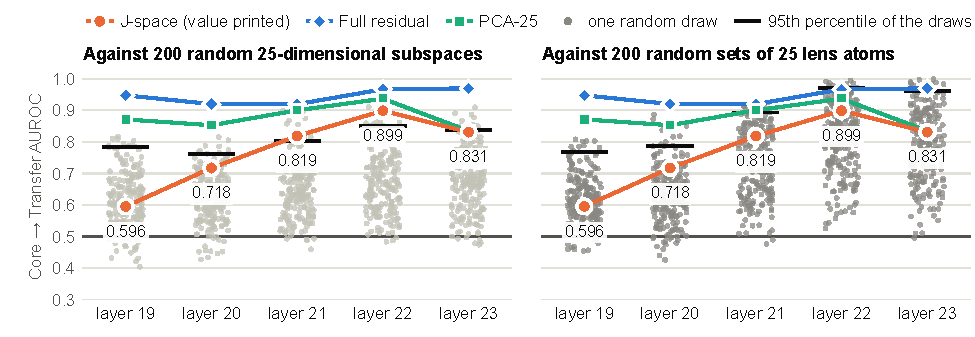
\includegraphics[width=\linewidth]{figs/fig_layers}
\caption{J-space against the two random nulls at each layer. A grey dot is one random draw; the black tick is the 95th
percentile of the 200 draws. Original condition, last token, $k=25$. The horizontal line is chance.}
\label{fig:layers}
\end{figure}

\paragraph{Caveats.} J-space is not empty: at layer 22 it reaches 0.929 and clears the random-subspace null, as many sets
of lens atoms do. Over all 35 cells of position and layer the rule is met in 1, at 50\% into the reply, where every
arm is near chance. Under swap it is met in 3 of 35 cells, at 50\% into the reply and at the last reply token, with scores
of 0.58 to 0.61. With 70 cells tested at the 5\% level, a few such cells are expected by chance.

% ---------------------------------------------------------------------------------------------------------- Finding 3
\findingbreak
\refstepcounter{finding}\label{f:within}
\subsection{Finding \thefinding: Without the instruction, colluders stand out within one set of scenarios but not across sets}

\paragraph{Question.} Once the instruction is out of the context, does the discussion itself still give the colluders away?

\paragraph{Answer.} Within Core, yes: 0.935 under swap when one domain is left out. Within Transfer, weakly: 0.667. From
Core to Transfer, no: 0.479 at the last token, with one weak exception early in the reply.

\paragraph{Why it matters.} This is the part of the result that is about behaviour. A detector of colluding behaviour, as
opposed to instructions, has to be built and tested here, and it has to be shown to transfer. Nothing we tested does so
clearly.

\begin{table}[H]\centering\small
\begin{tabular}{@{}lccccccccc@{}}\toprule
 & \multicolumn{3}{c}{Core $\to$ Transfer} & \multicolumn{3}{c}{Within Core (LODO)} & \multicolumn{3}{c}{Within Transfer (LOFO)}\\
\cmidrule(lr){2-4}\cmidrule(lr){5-7}\cmidrule(l){8-10}
Condition & Full & PCA-25 & J-space & Full & PCA-25 & J-space & Full & PCA-25 & J-space\\\midrule
Original & 0.945 & 0.879 & 0.773 & 1.000 & 1.000 & 0.988 & 0.974 & 0.898 & 0.866\\
Swap & 0.479 & 0.465 & 0.436 & 0.935 & 0.898 & 0.831 & 0.667 & 0.667 & 0.555\\
No system prompt & 0.488 & 0.466 & 0.475 & 0.934 & 0.889 & 0.822 & 0.631 & 0.609 & 0.605\\
Prompt only & 1.000 & 1.000 & 0.980 & 1.000 & 1.000 & 0.972 & 1.000 & 1.000 & 0.985\\
\bottomrule\end{tabular}

\caption{Primary AUROC under the three protocols, $k=25$, band mean over layers 19 to 23, at the last token (prompt only: at
the end of the system prompt). The left block is Figure~\ref{fig:controls}, left panel; the middle block its right panel.}
\label{tab:controls}
\end{table}

\paragraph{Evidence.} Table~\ref{tab:controls}, rows ``Swap'' and ``No system prompt''.
\begin{itemize}
\item \textbf{Within Core.} Under swap the full residual separates collusion from control episodes at 0.935, PCA-25 at
0.899 and J-space at 0.825. With no system prompt: 0.934, 0.889 and 0.822.
\item \textbf{Within Transfer.} Under swap 0.667, 0.667 and 0.547; with no system prompt 0.631, 0.609 and 0.565.
\item \textbf{Across.} 0.479 under swap and 0.488 with no system prompt, at the last token (Finding~\ref{f:instruction}).
\item \textbf{One weak exception across sets.} Under swap, PCA-25 read at 25\% into the reply transfers at 0.64 to 0.65 at
every layer (intervals between 0.53 and 0.75). The full residual at that position is at 0.488, and PCA with 8 or 100
components is at chance (0.475, 0.492). It is a lead, not a result.
\item \textbf{The within-Core signal is spread widely.} Under swap an average random 25-dimensional subspace reaches 0.86
to 0.88 within Core (20 draws per layer), more than J-space. The full residual is strongest when the whole reply is
averaged: 0.971.
\end{itemize}
What the within-Core signal is, we have not established. The transcripts offer candidates \src{Nov 8, CPU}. Colluders
argue for the target option: 73 of 100 voted for it, against 8 of 100 honest agents in the same episodes. Colluders use
fewer honesty and standards words in Core discussion: 8.3 per 1{,}000 words against 14.2. And a bag-of-words classifier on
the replies scores 0.853 within Core but 0.493 from Core to Transfer, the same pattern as the probe. The atom readout under
swap points the same way (Finding~\ref{f:atoms}): colluders' atoms more often include ``disagreed'' and ``argued''.

\paragraph{Caveats.}
\begin{itemize}
\item Within one set of scenarios, training and test episodes share a generation recipe, so a high score there does not
show a general signal. Under swap the context still holds messages that were written under the instruction.
\item The planned split of the activations by behaviour (colluders who voted for the target against those who did not) did
not run \notrun, so we cannot separate ``argues for the target'' from other differences.
\end{itemize}

% ---------------------------------------------------------------------------------------------------------- Finding 4
\findingbreak
\refstepcounter{finding}\label{f:atoms}
\subsection{Finding \thefinding: The J-space token readout echoes the instruction}

\paragraph{Question.} If we read the vocabulary tokens that colluders' J-space atoms stand for, do they describe the
collusion?

\paragraph{Answer.} Only with the instruction in the context. Most atoms are generic tokens shared by nearly every agent.
But colluders' atoms also include ``subtly'' and ``convincing'' on Core and ``disinformation'' and ``unethical'' on
Transfer.
With the instruction swapped out, no token differs by role on Transfer.

\paragraph{Why it matters.} This is J-space at its best: a plain-token readout that names the scheme. But it names the
instruction, as in Finding~\ref{f:instruction}, not colluding behaviour. It also corrects an earlier draft, which reported
stance words only.

\paragraph{Evidence.} Table~\ref{tab:atomroles}: layer 22, last token. Differences are in percentage points of agents.
\begin{itemize}
\item \textbf{Most atoms are the same for everyone.} The end-of-sequence token and an emphasis tag are among the atoms of
all 200 agents in Core collusion episodes, and ``decision'' of 186 (Table~\ref{tab:atoms}). The four word groups fixed in advance hold at most 1.1\% of the atoms in the
conversation.
\item \textbf{With the instruction present, colluders differ token by token.} On Core ``subtly'' is at $+61$ and
``recommending'' at $-65$. On Transfer ``disinformation'' is at $+62$ and ``subtly'' at $+51$. At layers 21 to 23
``subtly'' stays between $+50$ and $+76$ on both sets.
\item \textbf{Without the instruction the scheme words are gone.} Under swap, and with no system prompt, no token differs
by role on Transfer at any of the five layers. On Core tokens still differ, but they are words of disagreement, which fits
Finding~\ref{f:within}.
\item \textbf{Where it shows.} The instruction is visible in the atoms at the end of the system prompt already (on Core
``justifying'' at $+35$, ``scrutiny'' at $-32$). At 50\% into the reply no token differs by role in any cell.
\end{itemize}

\begin{table}[H]\centering\footnotesize
\begin{tabular}{@{}>{\raggedright\arraybackslash}p{0.105\linewidth}>{\raggedright\arraybackslash}p{0.2\linewidth}>{\raggedright\arraybackslash}p{0.225\linewidth}>{\raggedright\arraybackslash}p{0.2\linewidth}>{\raggedright\arraybackslash}p{0.13\linewidth}@{}}\toprule
 & \multicolumn{2}{l}{Instruction in context (original)} & \multicolumn{2}{l}{Instruction removed (swap)}\\
\cmidrule(r){2-3}\cmidrule(l){4-5}
 & Core & Transfer & Core & Transfer\\\midrule
Selected for more colluders & subtly ($+62$), convincing ($+50$), justifying ($+44$), lobbying ($+32$), arguing ($+28$) & disinformation ($+64$), ironically ($+61$), subtly ($+57$), misinformation ($+42$), unethical ($+39$) & disagreed ($+38$), nuanced ($+37$), suggested ($+36$), argued ($+30$), contradicts ($+29$) & none\\[2pt]
Selected for fewer colluders & recommending ($-59$), recommended ($-58$), recommendations ($-51$) & recommendations ($-49$), recommendation ($-49$), recommended ($-36$) & REJECT ($-48$), convincingly ($-46$), thankfully ($-44$) & none\\[2pt]
Tokens that differ & 30 or more & 30 or more & 30 or more & 0\\
\bottomrule\end{tabular}

\caption{Tokens that colluders and honest agents have among their atoms at different rates (layer 22, last token;
Benjamini--Hochberg at $q=0.05$). In brackets: the share of colluders with the token minus the share of honest agents in the
same episodes, in percentage points. Only tokens made of unaccented Latin letters are listed.}
\label{tab:atomroles}
\end{table}

\paragraph{Caveats.}
\begin{itemize}
\item Calling these ``scheme words'' is our reading of the token lists, made after seeing them. The word groups fixed in
advance did not capture them: they list exact word forms (``persuade'', ``argue''), and the atoms that differ are other
words. Of 320 tests of a group's share by role, 18 pass Benjamini--Hochberg, all with differences of at most 0.018.
\item The result files keep the 30 tokens with the smallest $p$ per cell. A token counts for an agent if it is among the
atoms of at least one of its turns. Readouts did not run at the \eot{} token \notrun.
\end{itemize}

% ---------------------------------------------------------------------------------------------------------- Finding 5
\findingbreak
\refstepcounter{finding}\label{f:position}
\subsection{Finding \thefinding: The transferable signal sits on the two tokens that close the turn}

\paragraph{Question.} Where in a turn can the probe read the signal that transfers?

\paragraph{Answer.} Only at the very end. At the last token of the reply text the full residual transfers at 0.517. One
token later, on \eot, it transfers at 0.780. One more token, on the newline that ends the turn, 0.945. Inside the reply it
is at chance.

\paragraph{Why it matters.} It says where the instruction-driven signal sits. It removes the hope that J-space would do
better at positions with more content: inside the reply no arm scores above 0.57. And it warns that results obtained within
one set of scenarios hide this, because there the signal is readable everywhere.

\paragraph{Evidence.} Figure~\ref{fig:positions}; every value is in Table~\ref{tab:posresults}.
\begin{itemize}
\item \textbf{Across sets, three consecutive tokens: 0.517, 0.780, 0.945.} Inside the reply the full residual scores 0.522,
0.527 and 0.571 at 25\%, 50\% and 75\%. The mean over all reply tokens gives 0.706.
\item \textbf{Within Core the position hardly matters.} The full residual scores 0.968 to 1.000 at every position.
\item \textbf{Within Transfer} it is in between: 0.50 to 0.59 inside the reply, 0.817 at the last reply token, 0.945 on
\eot{} and 0.974 at the last token.
\item \textbf{J-space} is below the 95th percentile of random subspaces at every position except the last token
(Finding~\ref{f:baselines}), and between 0.471 and 0.540 inside the reply.
\end{itemize}

\begin{figure}[H]\centering
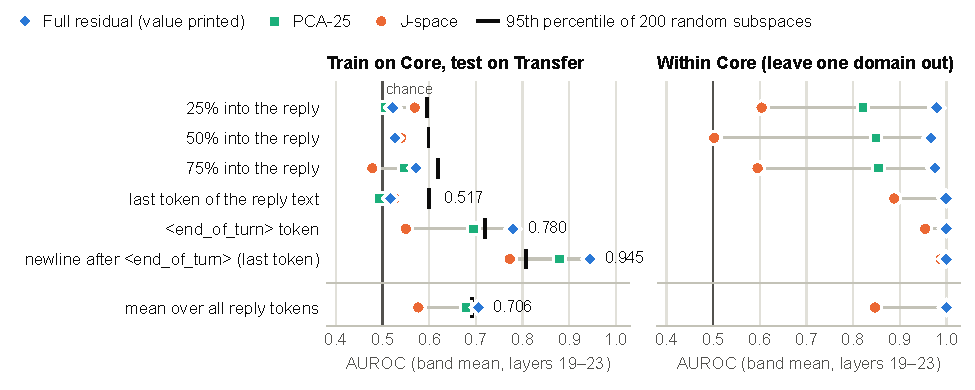
\includegraphics[width=\linewidth]{figs/fig_positions}
\caption{Read positions in the order they occur in a turn, with the mean over the reply below the line. Original condition,
$k=25$, band mean over layers 19 to 23.}
\label{fig:positions}
\end{figure}

\paragraph{Caveats.}
\begin{itemize}
\item We did not test why the signal sits on the closing tokens. One reading is that tokens inside the reply mostly encode
the local text, which differs between a committee discussion and a code review, while the closing tokens hold a summary of
the whole context. That is a guess.
\item The probe is fit on Core discussion turns and tested on Transfer final-vote turns, as in every earlier run. The two
kinds of turn differ, and that may matter most inside the reply.
\item The position called ``pre-vote'' in the code and in an earlier draft is the last reply token (Table~\ref{tab:positions}).
\end{itemize}

% ---------------------------------------------------------------------------------------------------------- Finding 6
\findingbreak
\refstepcounter{finding}\label{f:vocab}
\subsection{Finding \thefinding: The probe is not a vocabulary detector}

\paragraph{Question.} Does the probe fire on the words of collusion, or on the role?

\paragraph{Answer.} On the role. Honest agents whose system prompt carries a warning written in the colluders' own words
are separated from colluders perfectly by the full residual (1.000 at every layer). The warning moves them 4\% to 6\% of
the way toward the colluders. For J-space that share is 6\% to 24\%.

\paragraph{Why it matters.} It rules out the cheapest explanation of Finding~\ref{f:instruction}, that the probe matches
words in the prompt. What the probe reads is closer to being told to collude than to seeing the words.

\paragraph{Evidence.} Table~\ref{tab:mv}: the 50 warned control episodes of Step~8, original condition, last token; ranges
are over layers 19 to 23.
\begin{itemize}
\item \textbf{Warned agents are not mistaken for colluders.} Colluders against warned honest agents: 1.00 for the full
residual and PCA-25, 0.92 to 1.00 for J-space. At the episode level, collusion against warned episodes: 1.00.
\item \textbf{The warning is visible but small.} Warned against unwarned honest agents in the same episodes: 0.62 to 0.70
for the full residual (within-episode $p<0.001$), where 0.5 would mean the probe does not see the warning. Warned episodes
look slightly more like collusion than plain control episodes do (0.59 to 0.65).
\item \textbf{Echo ratio.} 0.04 to 0.06 for the full residual, 0.01 to 0.05 for PCA-25, 0.02 to 0.07 for random subspaces,
and 0.06 to 0.24 for J-space.
\end{itemize}

\begin{table}[H]\centering\small
\begin{tabularx}{\linewidth}{@{}Xcccc@{}}\toprule
 & Colluders vs & Warned vs & Echo & Collusion vs\\
Representation & warned agents & unwarned agents & ratio & warned episodes\\\midrule
Full residual & 1.00 & 0.62--0.70 & 0.04--0.06 & 1.00\\
J-space, 25 atoms & 0.92--1.00 & 0.51--0.80 & 0.06--0.24 & 0.95--1.00\\
PCA, 25 components & 1.00 & 0.55--0.62 & 0.01--0.05 & 1.00\\
Random 25-dimensional subspaces & 0.97 & 0.55--0.62 & 0.02--0.07 & n/a\\
\bottomrule\end{tabularx}

\caption{Matched-vocabulary control. The first two columns are AUROCs of agent scores; the echo ratio is the share of the
colluders' shift that the warning alone produces; the last column is the primary AUROC of the episode detectors. For random
subspaces: the mean over 20 draws, and the median for the echo ratio.}
\label{tab:mv}
\end{table}

\paragraph{Caveats.}
\begin{itemize}
\item J-space's echo ratio is 1.5 to 4.5 times the full residual's, partly because its gap between colluders and honest
agents is smaller, and that gap is the denominator. Measured as an AUROC, J-space separates warned from unwarned agents
about as well as the full residual does (0.51 to 0.80 against 0.62 to 0.70): more at layer 22 (0.80), less at layer 19
(0.51).
\item One warning text, 50 episodes, original condition only. The control did not run under swap or with no system prompt
\notrun.
\end{itemize}

% ---------------------------------------------------------------------------------------------------------- Finding 7
\findingbreak
\refstepcounter{finding}\label{f:steer}
\subsection{Finding \thefinding: Steering along J-space directions moves the vote logit, but mostly as any lens direction does}

\paragraph{Question.} If we push the residual along a J-space concept direction, does the vote change in a way that shows
these directions drive the collusive choice?

\paragraph{Answer.} The vote logit moves by up to 3.6 for honest agents, but at most 1\% of honest votes flip. Most of the
movement is generic: 20 random lens directions move honest agents by 2.2 to 2.9. Only ``deception'' and ``steering'' go
beyond all of them, by 0.7 logits at most.

\paragraph{Why it matters.} Against random Gaussian directions the result would have read as ``J-space concept directions
control the collusive vote''. Against a fair null most of it goes away. A steering claim made with lens directions needs a
lens-direction null.

\paragraph{Evidence.} Figure~\ref{fig:steering}: swap condition, layer 23, the largest strength ($\alpha=4$).
Table~\ref{tab:steer} has the values and Table~\ref{tab:steerfull} every run.
\begin{itemize}
\item \textbf{Against Gaussian directions every direction passes the four conditions of Step~10} at swap layer 23. At
layer 22 Benjamini--Hochberg fails, and under the original prompt three of the four concept directions move colluders the
wrong way.
\item \textbf{The four concept directions are nearly one direction.} Their pairwise cosines are 0.82 to 0.92, and each has
a cosine of 0.88 to 0.94 with the mean of all lens vectors, which a Gaussian direction does not share. ``Honesty'' moves
the vote the same way as ``deception''.
\item \textbf{Random lens directions share most of the effect.} They move honest agents by $+2.18$ to $+2.95$ and colluders
by $-1.23$ to $-0.80$. Deception is beyond all 20 draws by 0.66 (honest) and 0.37 (colluders), steering by 0.18 and 0.04
($p=1/21$). Coordination is beyond them for honest agents only, by 0.01; honesty is not.
\item \textbf{Votes barely move.} Honest agents start 8.6 logits from the target and at most 1\% cross. Colluders are
pushed off the target in at most 6\% of prompts by a concept direction and 10\% by the role direction; random Gaussian
directions reach 2\% and 9\%.
\end{itemize}

\begin{figure}[H]\centering
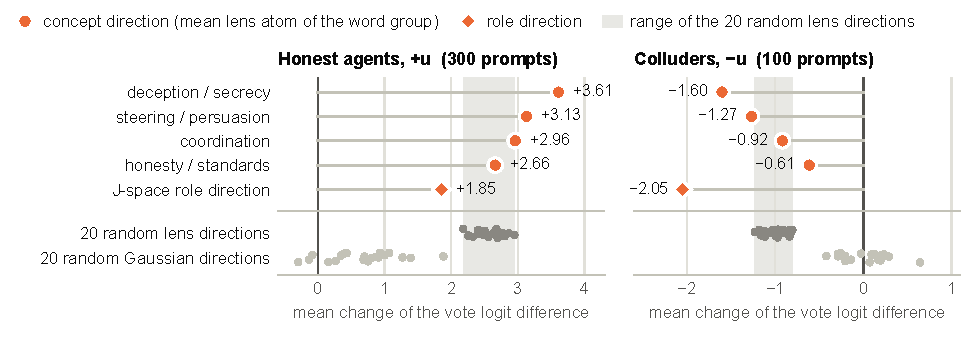
\includegraphics[width=\linewidth]{figs/fig_steering}
\caption{Mean change of the vote logit difference, in logits, at the largest strength; swap condition, layer 23. The grey
band is the range of the 20 random lens directions. A concept direction is specific only where it falls outside the band.}
\label{fig:steering}
\end{figure}

\paragraph{Caveats.} With 20 draws the smallest possible $p$ is $1/21$, so a sharper statement needs more draws. The lens
null ran at one layer and one condition, and not for the role direction. Steered passes reuse a cached prefix and differ
from full passes by up to 0.13 logits. The steering scale, the median length of $h_J$, is our own choice. The scale and
the role direction come from the November~9 decomposition \src{Nov 9 decomposition} and were not recomputed; the concept
directions and the random lens directions do not depend on the decomposition.

% =====================================================================================================================
\section{What did not run}\label{sec:notrun}
\begin{itemize}
\item \textbf{Steering with the original prompt at layer 23.} The steering job hit its 4-hour limit after three of the four
planned runs.
\item \textbf{The paired-interval half of the rule for random subspaces} (Step~7). The random draws were scored without the
bootstrap. The one-sided $p$ against the 200 draws is reported instead.
\item \textbf{The matched-vocabulary control under swap and with no system prompt.} The warned episodes were extracted for
the original and prompt-only conditions only.
\item \textbf{Atom readouts at the \eot{} token and at other reply positions.} They ran at the last token, the last reply
token, 50\% into the reply, and the end of the system prompt.
\item \textbf{The split of the activations by behaviour} (colluders who voted for the target against those who did not).
It was planned on November~8 and exists for the text only (Appendix~\ref{app:earlier}).
\item \textbf{A larger lens null for steering,} at more layers and for the role direction. It ran with 20 draws at swap
layer 23.
\item \textbf{An end-to-end run of \jlens{} on the model} (Section~\ref{sec:impl}).
\item \textbf{Steering with the present decomposition.} The role direction and the strength of the steering runs come from
the November~9 decomposition; the runs were not repeated.
\item \textbf{Sizes other than 25 away from the headline cell.} With the whole-vocabulary pursuit, $k=8$, 50 and 100 ran at
the last token of the original condition only.
\item \textbf{Other models.} No Jacobian lens is published for the other three models with NARCBench activations.
\item \textbf{Collusion without an instruction.} The benchmark only has instructed collusion.
\end{itemize}
All 80 cells of the sweep ran at $k=25$ (16 pairs of condition and read position, five layers each), and the 15 cells
of the three other sizes at the headline cell. The steering runs failed on the first GPU job with an out-of-memory error in our own loop and were rerun after
the fix (Appendix~\ref{app:run}).

\section{Limitations}\label{sec:limits}
\begin{itemize}
\item \textbf{Scope.} One model, one published lens, one run, and collusion that is instructed.
\item \textbf{The decomposition is our implementation.} No reference code exists for it; Section~\ref{sec:impl} lists the
choices the paper leaves open and tests the main ones on one cell. One of them, a shortlist of candidate tokens for the
pursuit, moved the headline score by 0.05. The J-space numbers therefore carry an uncertainty of that order from the
implementation alone, next to the sampling intervals.
\item \textbf{The rule against the random nulls is per layer.} Averaged over the five layers, J-space is above nearly
every random draw (Finding~\ref{f:baselines}). The rule was fixed per layer before the run and we did not change it.
\item \textbf{Train and test turns differ.} Probes are fit on Core discussion turns and tested on Transfer final-vote turns.
\item \textbf{Many cells.} There are 35 cells per condition at $k=25$, so single cells clear a bar by chance.
\item \textbf{The first run was not reproduced exactly.} The activations were regenerated (seven positions, bf16). The full
residual now transfers at 0.945 where the first run had 0.902; the profile over layers and arms is the same.
\item \textbf{The reading of the tokens in Finding~\ref{f:atoms} was made after seeing them.} The word groups were fixed in
advance, but their choice is ours.
\item \textbf{Text baselines} are bag-of-words models. Claims about related work are from an abstract or second-hand
(Appendix~\ref{app:related}).
\end{itemize}

\section{Conclusion and recommendations}\label{sec:next}
Should J-space be the standard? No. As a detector it clears none of the three bars set for it
(Finding~\ref{f:baselines}).
As a readout it does show the scheme in plain tokens at the end of a turn (Finding~\ref{f:atoms}), which is its most
favourable result here. But what it shows is the instruction, fixed word groups do not capture it, and its concept
directions do not steer the vote specifically (Finding~\ref{f:steer}). We recommend the following.
\begin{enumerate}
\item \textbf{Keep the full-residual probe as the reference detector,} and describe it as an instruction detector on this
benchmark.
\item \textbf{Report every detector next to its swap and prompt-only scores.} A detector claim on NARCBench without them
cannot be told apart from reading the instruction.
\item \textbf{Treat collusion without an instruction as the real test.} On the instructed benchmark the instruction is the
signal. The within-set signal of Finding~\ref{f:within} is where a behaviour detector would start, and it has to transfer.
\item \textbf{Use a lens-direction null} for any steering claim made with lens vectors.
\item \textbf{If J-space is used for reading, read token by token} at the last token of a turn, with a swap control, and not
through fixed word lists.
\item \textbf{Keep the lens and its application tied to Anthropic's reference implementation,} and state which solver and
which search were used for the decomposition, since none is released: a shortlist of candidate tokens alone moved our
headline score by 0.05.
\end{enumerate}

\begin{thebibliography}{9}
\bibitem{gurnee2026workspace} W.~Gurnee et al. Verbalizable Representations Form a Global Workspace in Language Models.
Transformer Circuits Thread, 2026. \url{https://transformer-circuits.pub/2026/workspace/index.html}. arXiv:2607.15495.
\bibitem{jlens} Anthropic. \texttt{jlens}: Jacobian lens, reference implementation (companion code of
\cite{gurnee2026workspace}), version 0.1.0, commit \texttt{581d398}, 2026.
\url{https://github.com/anthropics/jacobian-lens}.
\bibitem{neuronpedialens} Neuronpedia. Jacobian lens for \texttt{google/gemma-2-9b-it}, fitted with \texttt{jlens} on
WikiText-103, June 2026. Hugging Face repository \texttt{neuronpedia/jacobian-lens}, file
\texttt{gemma-2-9b-it/jlens/Salesforce-wikitext/gemma-2-9b-it\_jacobian\_lens.pt}.
\bibitem{rose2026narcbench} J.~Rose et al. Detecting Multi-Agent Collusion Through Multi-Agent Interpretability.
arXiv:2604.01151, 2026.
\bibitem{molinari2026collusion} M.~Molinari and G.~Bettineschi. Multi-Agent Collusion and the J-Space. arXiv:2611.02153,
2026.
\bibitem{gemma2} Gemma Team. Gemma 2: Improving Open Language Models at a Practical Size. arXiv:2408.00118, 2024.
\bibitem{blumensath2008} T.~Blumensath and M.~E.~Davies. Gradient pursuits. \emph{IEEE Transactions on Signal Processing},
56(6):2370--2382, 2008.
\bibitem{benjamini1995} Y.~Benjamini and Y.~Hochberg. Controlling the false discovery rate: a practical and powerful
approach to multiple testing. \emph{Journal of the Royal Statistical Society: Series B}, 57(1):289--300, 1995.
\end{thebibliography}

% =====================================================================================================================
\clearpage
\appendix
\section{Tables behind the findings}\label{app:tables}
The code names of the read positions are those of Table~\ref{tab:positions}; \tok{prevote} is the last token of the reply
text. ``J-space'' is the non-negative combination of the pursuit's atoms (the primary form of Step~4), ``J span'' the
projection onto the span of exactly $k$ vectors, ``Compl.'' the complement. Over the 35 cells of position and layer in the original condition, PCA-25 is
reliably better than J-space in 6 and J-space in none (paired 95\% bootstrap intervals).

\begin{table}[H]\centering\small
\resizebox{\linewidth}{!}{\begin{tabular}{@{}lcccccc@{}}\toprule
$k$ & J-space & Span of exactly $k$ & PCA-$k$ & Random subspaces (p95) & Random lens atoms (p95) & Full residual\\\midrule
8 & 0.765 & 0.764 & 0.833 & 0.771 & 0.842 & 0.945\\
25 & 0.819 & 0.815 & 0.879 & 0.808 & 0.875 & 0.945\\
50 & 0.814 & 0.797 & 0.928 & 0.851 & 0.895 & 0.945\\
100 & 0.814 & 0.808 & 0.938 & 0.896 & 0.925 & 0.945\\
\bottomrule\end{tabular}
}
\caption{Finding~\ref{f:baselines}: the comparison at four subspace sizes. Core$\to$Transfer, original condition, last token,
band means; p95 is the 95th percentile of 200 draws.}
\label{tab:ksweep}
\end{table}

\begin{table}[H]\centering\small
\begin{tabular}{@{}lc@{\hskip 2.2em}lc@{}}\toprule
\multicolumn{2}{@{}l}{Last token (newline after \texttt{<end\_of\_turn>})} & \multicolumn{2}{l}{Last token of the reply text}\\
Atom (vocabulary token) & Agents & Atom (vocabulary token) & Agents\\\midrule
\texttt{\textvisiblespace{}decision} & 189 & \texttt{<eos>} & 200\\
\texttt{\textvisiblespace{}prioritizing} & 177 & \texttt{\textvisiblespace{}prioriti} & 200\\
\texttt{<eos>} & 161 & \texttt{\textvisiblespace{}acknowledging} & 199\\
\texttt{\textvisiblespace{}eloquently} & 161 & \texttt{\textvisiblespace{}pungkasnya} & 199\\
\texttt{\textvisiblespace{}diría} & 161 & \texttt{.} & 198\\
\texttt{\textvisiblespace{}discussions} & 155 & \texttt{\textvisiblespace{}\textvisiblespace{}} & 198\\
\texttt{\textvisiblespace{}recommendation} & 154 & \texttt{\textvisiblespace{}concludes} & 197\\
\texttt{\textvisiblespace{}recommendations} & 149 & \texttt{\textvisiblespace{}respectfully} & 195\\
\bottomrule\end{tabular}

\caption{Finding~\ref{f:atoms}: the most common atoms at layer 22 and the number of the 200 agents in Core collusion
episodes that have each in at least one of their three discussion turns. \tok{\textvisiblespace} marks a leading space.
Characters that the fonts of this paper lack are printed as Unicode code points: [U+202F] is a narrow no-break space,
[U+4E86][U+55CE] are two Chinese characters.}
\label{tab:atoms}
\end{table}

\begin{table}[H]\centering\small
\resizebox{\linewidth}{!}{\begin{tabular}{@{}llcccccc@{}}\toprule
 & & \multicolumn{4}{c}{Core $\to$ Transfer} & \multicolumn{2}{c}{Full residual, within a split}\\
\cmidrule(lr){3-6}\cmidrule(l){7-8}
Read position & Code name & Full & PCA-25 & J-space & Random p95 & Core LODO & Transfer LOFO\\\midrule
25\% into the reply & \texttt{frac25} & 0.522 & 0.507 & 0.569 & 0.595 & 0.980 & 0.587\\
50\% into the reply & \texttt{frac50} & 0.527 & 0.538 & 0.540 & 0.598 & 0.968 & 0.499\\
75\% into the reply & \texttt{frac75} & 0.571 & 0.546 & 0.478 & 0.619 & 0.975 & 0.550\\
last token of the reply text & \texttt{prevote} & 0.517 & 0.494 & 0.526 & 0.600 & 0.999 & 0.817\\
\texttt{<end\_of\_turn>} token & \texttt{eot} & 0.780 & 0.695 & 0.550 & 0.719 & 1.000 & 0.945\\
newline after \texttt{<end\_of\_turn>} (last token) & \texttt{last} & 0.945 & 0.879 & 0.773 & 0.808 & 1.000 & 0.974\\
mean over all reply tokens & \texttt{reply\_mean} & 0.706 & 0.679 & 0.577 & 0.691 & 1.000 & 0.900\\
\bottomrule\end{tabular}
}
\caption{Finding~\ref{f:position}: primary AUROC by read position, original condition, $k=25$, band mean. ``Random p95'' is
the 95th percentile of 200 random subspaces.}
\label{tab:posresults}
\end{table}

\begin{table}[H]\centering\small
\resizebox{\linewidth}{!}{\begin{tabular}{@{}lccccc@{}}\toprule
 & \multicolumn{2}{c}{Honest agents, $+u$} & \multicolumn{2}{c}{Colluders, $-u$} & Beyond all 20 random\\
\cmidrule(lr){2-3}\cmidrule(lr){4-5}
Direction $u$ & $\Delta y$ & votes flipped & $\Delta y$ & votes flipped & lens directions?\\\midrule
deception / secrecy & $+3.61$ & 0\% & $-1.60$ & 3\% & both groups\\
steering / persuasion & $+3.13$ & 0\% & $-1.27$ & 3\% & both groups\\
coordination & $+2.96$ & 1\% & $-0.92$ & 3\% & honest agents only\\
honesty / standards & $+2.66$ & 0\% & $-0.61$ & 2\% & neither group\\
J-space role direction & $+1.85$ & 0\% & $-2.05$ & 10\% & not tested\\
\midrule
20 random lens directions (range) & $+2.18$ to $+2.95$ & up to 1\% & $-1.23$ to $-0.80$ & up to 3\% & \\
20 random Gaussian directions (range) & $-0.30$ to $+1.88$ & up to 2\% & $-0.42$ to $+0.64$ & up to 9\% & \\
\bottomrule\end{tabular}
}
\caption{Finding~\ref{f:steer}: steering at $\alpha=4$, swap condition, layer 23. $\Delta y$ is the mean change of
$\mathrm{logit}(\text{target})-\mathrm{logit}(\text{fair})$. A vote flips when $y$ changes sign: toward the target for
honest agents, away from it for colluders.}
\label{tab:steer}
\end{table}

\begin{table}[H]\centering\footnotesize\setlength{\tabcolsep}{4pt}
\resizebox{\linewidth}{!}{\begin{tabular}{llcccccccc}\toprule
Cond. & Position & Full & J fill & J pursuit & Compl. & PCA-$k$ & Rand.\ sub.\ mean (p95) & Rand.\ atoms p95 & Layers clearing both\\\midrule
original & last & 0.945 & 0.773 & 0.765 & 0.941 & 0.879 & 0.650 (0.808) & 0.875 & 0/5\\
 & eot & 0.780 & 0.550 & 0.584 & 0.768 & 0.695 & 0.584 (0.719) & 0.763 & 0/5\\
 & prevote & 0.517 & 0.526 & 0.535 & 0.520 & 0.494 & 0.512 (0.600) & 0.588 & 0/5\\
 & reply\_mean & 0.706 & 0.577 & 0.575 & 0.710 & 0.679 & 0.610 (0.691) & 0.658 & 0/5\\
 & frac25 & 0.522 & 0.569 & 0.517 & 0.521 & 0.507 & 0.500 (0.595) & 0.580 & 2/5\\
 & frac50 & 0.527 & 0.540 & 0.536 & 0.529 & 0.538 & 0.502 (0.598) & 0.596 & 0/5\\
 & frac75 & 0.571 & 0.478 & 0.461 & 0.567 & 0.546 & 0.519 (0.619) & 0.602 & 0/5\\
\midrule
swap & last & 0.479 & 0.436 & 0.473 & 0.468 & 0.465 & 0.508 (0.609) & 0.595 & 0/5\\
 & eot & 0.491 & 0.492 & 0.513 & 0.489 & 0.491 & 0.512 (0.611) & 0.594 & 0/5\\
 & prevote & 0.469 & 0.515 & 0.537 & 0.477 & 0.479 & 0.501 (0.587) & 0.572 & 1/5\\
 & reply\_mean & 0.554 & 0.585 & 0.579 & 0.555 & 0.541 & 0.565 (0.649) & 0.627 & 0/5\\
 & frac25 & 0.488 & 0.508 & 0.531 & 0.482 & 0.643 & 0.514 (0.612) & 0.596 & 0/5\\
 & frac50 & 0.519 & 0.537 & 0.559 & 0.518 & 0.610 & 0.508 (0.608) & 0.602 & 0/5\\
 & frac75 & 0.573 & 0.471 & 0.469 & 0.564 & 0.514 & 0.505 (0.601) & 0.592 & 0/5\\
\bottomrule\end{tabular}
}
\caption{Core$\to$Transfer primary AUROC at $k=25$, band mean over layers 19 to 23, per condition and read position.
``Layers clearing both'' counts the layers at which J-space is above the 95th percentile of both random nulls.}
\end{table}

\begin{table}[H]\centering\footnotesize
\resizebox{\linewidth}{!}{\begin{tabular}{lcccccccc}\toprule
Layer & Full & J fill & J pursuit & PCA-$k$ & Rand.\ sub.\ p95 & Rand.\ atoms p95 & $p$ vs rand.\ sub. & Clears both\\\midrule
19 & 0.948 [0.91, 0.98] & 0.596 [0.50, 0.69] & 0.598 & 0.871 & 0.783 & 0.767 & 0.597 & --\\
20 & 0.920 [0.88, 0.96] & 0.718 [0.64, 0.79] & 0.724 & 0.853 & 0.763 & 0.786 & 0.149 & --\\
21 & 0.919 [0.88, 0.95] & 0.819 [0.76, 0.87] & 0.773 & 0.900 & 0.803 & 0.893 & 0.040 & --\\
22 & 0.967 [0.95, 0.99] & 0.899 [0.85, 0.94] & 0.924 & 0.937 & 0.851 & 0.969 & 0.010 & --\\
23 & 0.970 [0.95, 0.99] & 0.831 [0.77, 0.89] & 0.806 & 0.835 & 0.838 & 0.961 & 0.075 & --\\
\bottomrule\end{tabular}
}
\caption{Per layer, original condition, last token, $k=25$, with 95\% episode-bootstrap intervals and the one-sided $p$ of
J-space against the 200 random subspaces.}
\end{table}

\begin{table}[H]\centering\footnotesize
\resizebox{\linewidth}{!}{\begin{tabular}{lcccccccc}\toprule
Layer & Full & J fill & J pursuit & PCA-$k$ & Rand.\ sub.\ p95 & Rand.\ atoms p95 & $p$ vs rand.\ sub. & Clears both\\\midrule
19 & 0.450 [0.35, 0.55] & 0.417 [0.31, 0.52] & 0.465 & 0.451 & 0.606 & 0.617 & 0.970 & --\\
20 & 0.457 [0.36, 0.55] & 0.382 [0.28, 0.49] & 0.483 & 0.461 & 0.625 & 0.586 & 1.000 & --\\
21 & 0.484 [0.39, 0.58] & 0.475 [0.39, 0.56] & 0.534 & 0.486 & 0.604 & 0.572 & 0.657 & --\\
22 & 0.460 [0.38, 0.55] & 0.457 [0.38, 0.54] & 0.445 & 0.481 & 0.588 & 0.597 & 0.831 & --\\
23 & 0.542 [0.45, 0.64] & 0.447 [0.34, 0.55] & 0.440 & 0.443 & 0.620 & 0.604 & 0.900 & --\\
\bottomrule\end{tabular}
}
\caption{The same under swap: every arm at chance at every layer.}
\end{table}

\begin{table}[H]\centering\footnotesize
\begin{tabular}{lcccccccc}\toprule
Layer & \multicolumn{2}{c}{original/last} & \multicolumn{2}{c}{swap/last} & \multicolumn{2}{c}{nosys/last} & \multicolumn{2}{c}{prompt\_only/prompt\_end}\\
 & Full & J fill & Full & J fill & Full & J fill & Full & J fill\\\midrule
19 & 0.948 & 0.596 & 0.450 & 0.417 & 0.503 & 0.504 & 1.000 & 0.985\\
20 & 0.920 & 0.718 & 0.457 & 0.382 & 0.472 & 0.414 & 1.000 & 0.998\\
21 & 0.919 & 0.819 & 0.484 & 0.475 & 0.474 & 0.501 & 1.000 & 0.997\\
22 & 0.967 & 0.899 & 0.460 & 0.457 & 0.490 & 0.496 & 1.000 & 0.968\\
23 & 0.970 & 0.831 & 0.542 & 0.447 & 0.504 & 0.462 & 1.000 & 0.952\\
\bottomrule\end{tabular}

\caption{Core$\to$Transfer primary AUROC per layer for the four conditions, full residual and J-space at $k=25$.}
\end{table}

\begin{table}[H]\centering\footnotesize
\resizebox{\linewidth}{!}{\begin{tabular}{lcccccccc}\toprule
$k$ & Full & J fill & J pursuit & Compl. & PCA-$k$ & Rand.\ sub.\ p95 & Rand.\ atoms p95 & J fill $-$ PCA (95\% CI)\\\midrule
8 & 0.945 & 0.740 & 0.740 & 0.944 & 0.831 & 0.771 & 0.842 & [-0.08, 0.02] (L22)\\
25 & 0.945 & 0.773 & 0.765 & 0.941 & 0.879 & 0.808 & 0.875 & [-0.09, 0.02] (L22)\\
50 & 0.945 & 0.762 & 0.766 & 0.938 & 0.928 & 0.851 & 0.895 & [-0.10, -0.00] (L22)\\
100 & 0.945 & 0.807 & 0.766 & 0.938 & 0.938 & 0.896 & 0.925 & [-0.08, 0.00] (L22)\\
\bottomrule\end{tabular}
}
\caption{$k$ sweep with all arms, original condition, last token, band mean. The paired interval of J-space minus PCA-$k$
is for layer 22.}
\end{table}

\begin{table}[H]\centering\footnotesize\setlength{\tabcolsep}{4pt}
\resizebox{\linewidth}{!}{\begin{tabular}{llccccccccc}\toprule
Cond. & Pos. & \multicolumn{3}{c}{Full} & \multicolumn{3}{c}{J fill $k{=}25$} & \multicolumn{3}{c}{PCA-25}\\
 & & LODO & C$\to$T & LOFO & LODO & C$\to$T & LOFO & LODO & C$\to$T & LOFO\\\midrule
original & last & 1.000 & 0.945 & 0.974 & 0.988 & 0.773 & 0.866 & 1.000 & 0.879 & 0.898\\
 & prevote & 0.999 & 0.517 & 0.817 & 0.888 & 0.526 & 0.629 & 0.999 & 0.494 & 0.621\\
swap & last & 0.935 & 0.479 & 0.667 & 0.831 & 0.436 & 0.555 & 0.898 & 0.465 & 0.667\\
 & prevote & 0.908 & 0.469 & 0.649 & 0.750 & 0.515 & 0.582 & 0.900 & 0.479 & 0.626\\
nosys & last & 0.934 & 0.488 & 0.631 & 0.822 & 0.475 & 0.605 & 0.889 & 0.466 & 0.609\\
prompt\_only & prompt\_end & 1.000 & 1.000 & 1.000 & 0.972 & 0.980 & 0.985 & 1.000 & 1.000 & 1.000\\
\bottomrule\end{tabular}
}
\caption{The three protocols per condition, band mean: Core leave-one-domain-out (LODO), Core$\to$Transfer (C$\to$T) and
Transfer leave-one-family-out (LOFO).}
\end{table}

\begin{table}[H]\centering\footnotesize\setlength{\tabcolsep}{4pt}
\resizebox{\linewidth}{!}{\begin{tabular}{llcccccc}\toprule
Cell & Arm & Coll.\ vs warned & Warned vs unwarned ($p$) & Warned vs control & Echo & Ep.\ warned vs control & Ep.\ coll.\ vs warned\\\midrule
original/last/L22 & Full & 1.000 & 0.694 (0.00) & 0.612 & 0.05 & 0.632 & 1.000\\
 & J-space $k{=}25$ & 0.989 & 0.803 (0.00) & 0.812 & 0.24 & 0.844 & 0.996\\
 & PCA-25 & 0.999 & 0.572 (0.00) & 0.525 & 0.02 & 0.527 & 1.000\\
 & Random 25-dim, mean of 20 (echo: median) & 0.973 & 0.587 & 0.555 & 0.03 & 0.557 & n/a\\
\midrule
original/prevote/L22 & Full & 1.000 & 0.736 (0.00) & 0.741 & 0.13 & 0.738 & 1.000\\
 & J-space $k{=}25$ & 0.923 & 0.557 (0.03) & 0.592 & 0.14 & 0.546 & 0.950\\
 & PCA-25 & 0.998 & 0.718 (0.00) & 0.745 & 0.17 & 0.700 & 0.999\\
 & Random 25-dim, mean of 20 (echo: median) & 0.890 & 0.615 & 0.605 & 0.16 & 0.563 & n/a\\
\bottomrule\end{tabular}
}
\caption{Matched-vocabulary control at layer 22, at the last token and at the last reply token, scored out of fold.}
\end{table}

\begin{table}[H]\centering\footnotesize
\resizebox{\linewidth}{!}{\begin{tabular}{llcccc}\toprule
Cell & Group & Colluder & Honest (same ep.) & Control & BH $p$ (within ep.)\\\midrule
swap/frac50/L22 & deception/secrecy & 0.0000 & 0.0000 & 0.0000 & 1.000\\
 & coordination & 0.0000 & 0.0001 & 0.0008 & 1.000\\
 & steering/persuasion & 0.0000 & 0.0000 & 0.0001 & 1.000\\
 & honesty/standards & 0.0056 & 0.0067 & 0.0082 & 1.000\\
\multicolumn{6}{l}{\footnotesize most common atoms (Core): \texttt{\textvisiblespace{}potentially} (153), \texttt{\textvisiblespace{}prioritizing} (144), \texttt{\textvisiblespace{}prioriti} (118), \texttt{\textvisiblespace{}impactful} (115), \texttt{\textvisiblespace{}potential} (110), \texttt{\textvisiblespace{}ethically} (104)}\\
\midrule
swap/last/L22 & deception/secrecy & 0.0000 & 0.0000 & 0.0000 & 1.000\\
 & coordination & 0.0000 & 0.0000 & 0.0000 & 1.000\\
 & steering/persuasion & 0.0007 & 0.0011 & 0.0007 & 1.000\\
 & honesty/standards & 0.0000 & 0.0000 & 0.0000 & 1.000\\
\multicolumn{6}{l}{\footnotesize most common atoms (Core): \texttt{<eos>} (200), \texttt{\textvisiblespace{}decision} (200), \texttt{<em>} (200), \texttt{\textvisiblespace{}prioritizing} (199), \texttt{.\textrm{[U+202F]}} (199), \texttt{.**} (198)}\\
\midrule
swap/prevote/L22 & deception/secrecy & 0.0000 & 0.0000 & 0.0000 & 1.000\\
 & coordination & 0.0000 & 0.0000 & 0.0000 & 1.000\\
 & steering/persuasion & 0.0000 & 0.0000 & 0.0000 & 1.000\\
 & honesty/standards & 0.0000 & 0.0000 & 0.0002 & 1.000\\
\multicolumn{6}{l}{\footnotesize most common atoms (Core): \texttt{<eos>} (200), \texttt{.”} (200), \texttt{'.} (198), \texttt{\textvisiblespace{}prioriti} (197), \texttt{\textvisiblespace{}acknowledging} (193), \texttt{\textvisiblespace{}despite} (192)}\\
\midrule
original/last/L22 & deception/secrecy & 0.0004 & 0.0002 & 0.0000 & 1.000\\
 & coordination & 0.0000 & 0.0000 & 0.0000 & 1.000\\
 & steering/persuasion & 0.0011 & 0.0013 & 0.0007 & 1.000\\
 & honesty/standards & 0.0000 & 0.0000 & 0.0000 & 1.000\\
\multicolumn{6}{l}{\footnotesize most common atoms (Core): \texttt{<eos>} (200), \texttt{<em>} (200), \texttt{.\textrm{[U+202F]}} (196), \texttt{\textvisiblespace{}decision} (186), \texttt{.**} (180), \texttt{\textvisiblespace{}prioritizing} (165)}\\
\midrule
original/prevote/L22 & deception/secrecy & 0.0000 & 0.0000 & 0.0000 & 1.000\\
 & coordination & 0.0000 & 0.0000 & 0.0000 & 1.000\\
 & steering/persuasion & 0.0000 & 0.0000 & 0.0000 & 1.000\\
 & honesty/standards & 0.0000 & 0.0000 & 0.0002 & 1.000\\
\multicolumn{6}{l}{\footnotesize most common atoms (Core): \texttt{<eos>} (200), \texttt{.”} (200), \texttt{'.} (198), \texttt{\textvisiblespace{}prioriti} (197), \texttt{\textvisiblespace{}acknowledging} (196), \texttt{\textvisiblespace{}despite} (196)}\\
\bottomrule\end{tabular}
}
\caption{Share of the four word groups among the $k=25$ atoms at layer 22, mean per agent over its three Core discussion
turns, with Benjamini--Hochberg adjusted within-episode permutation $p$.}
\end{table}

\begin{table}[H]\centering\footnotesize
\resizebox{\linewidth}{!}{\begin{tabular}{lllccccccccc}\toprule
Run & Direction & Group ($n$) & $\Delta y$ at $\alpha{=}1$ & $\alpha{=}2$ & $\alpha{=}4$ & Flips $\alpha{=}2$ & $\alpha{=}4$ & Sign & $>$ rand.\ p95 & BH & All bars\\\midrule
original L22 & deception\_secrecy & colluder (100) & -0.01 & -0.12 & -0.47 & 0.03 & 0.06 & -- & -- & -- & --\\
 & deception\_secrecy & honest (300) & 0.83 & 1.87 & 3.21 & 0.00 & 0.00 & $\checkmark$ & $\checkmark$ & -- & --\\
 & coordination & colluder (100) & 0.11 & 0.17 & 0.20 & 0.01 & 0.03 & -- & -- & -- & --\\
 & coordination & honest (300) & 0.74 & 1.76 & 2.49 & 0.00 & 0.00 & $\checkmark$ & $\checkmark$ & -- & --\\
 & steering\_persuasion & colluder (100) & 0.10 & 0.13 & 0.05 & 0.01 & 0.04 & -- & -- & -- & --\\
 & steering\_persuasion & honest (300) & 0.79 & 1.82 & 2.68 & 0.00 & 0.00 & $\checkmark$ & $\checkmark$ & -- & --\\
 & honesty\_standards & colluder (100) & 0.19 & 0.29 & 0.38 & 0.01 & 0.03 & -- & -- & -- & --\\
 & honesty\_standards & honest (300) & 0.73 & 1.73 & 2.41 & 0.00 & 0.01 & $\checkmark$ & $\checkmark$ & -- & --\\
 & J role probe & colluder (100) & -0.14 & -0.31 & -0.66 & 0.00 & 0.01 & $\checkmark$ & -- & -- & --\\
 & J role probe & honest (300) & 0.17 & 0.55 & 1.90 & 0.00 & 0.00 & $\checkmark$ & -- & -- & --\\
\multicolumn{12}{l}{\footnotesize colluder: baseline $y_0$ mean 3.54, share with $y_0>0$ 0.73; 20 random directions at $\alpha{=}4$: mean $\Delta y$ from -0.95 to 0.38}\\
\multicolumn{12}{l}{\footnotesize honest: baseline $y_0$ mean -8.63, share with $y_0>0$ 0.05; 20 random directions at $\alpha{=}4$: mean $\Delta y$ from -0.11 to 1.94}\\
\midrule
swap L22 & deception\_secrecy & colluder (100) & -0.35 & -0.58 & -0.88 & 0.01 & 0.03 & $\checkmark$ & $\checkmark$ & -- & --\\
 & deception\_secrecy & honest (300) & 0.84 & 1.91 & 3.25 & 0.00 & 0.00 & $\checkmark$ & $\checkmark$ & -- & --\\
 & coordination & colluder (100) & -0.18 & -0.29 & -0.33 & 0.00 & 0.00 & $\checkmark$ & -- & -- & --\\
 & coordination & honest (300) & 0.76 & 1.79 & 2.53 & 0.00 & 0.00 & $\checkmark$ & $\checkmark$ & -- & --\\
 & steering\_persuasion & colluder (100) & -0.27 & -0.43 & -0.61 & 0.00 & 0.02 & $\checkmark$ & -- & -- & --\\
 & steering\_persuasion & honest (300) & 0.81 & 1.85 & 2.71 & 0.00 & 0.00 & $\checkmark$ & $\checkmark$ & -- & --\\
 & honesty\_standards & colluder (100) & -0.19 & -0.28 & -0.26 & 0.00 & 0.02 & $\checkmark$ & -- & -- & --\\
 & honesty\_standards & honest (300) & 0.74 & 1.75 & 2.45 & 0.00 & 0.01 & $\checkmark$ & $\checkmark$ & -- & --\\
 & J role probe & colluder (100) & -0.41 & -0.82 & -1.54 & 0.03 & 0.10 & $\checkmark$ & $\checkmark$ & -- & --\\
 & J role probe & honest (300) & 0.51 & 1.11 & 2.38 & 0.01 & 0.01 & $\checkmark$ & $\checkmark$ & -- & --\\
\multicolumn{12}{l}{\footnotesize colluder: baseline $y_0$ mean -3.85, share with $y_0>0$ 0.24; 20 random directions at $\alpha{=}4$: mean $\Delta y$ from -0.63 to 0.69}\\
\multicolumn{12}{l}{\footnotesize honest: baseline $y_0$ mean -8.63, share with $y_0>0$ 0.05; 20 random directions at $\alpha{=}4$: mean $\Delta y$ from -0.11 to 1.99}\\
\midrule
swap L23 & deception\_secrecy & colluder (100) & -0.52 & -0.98 & -1.60 & 0.01 & 0.03 & $\checkmark$ & $\checkmark$ & $\checkmark$ & $\checkmark$\\
 & deception\_secrecy & honest (300) & 1.06 & 2.33 & 3.61 & 0.00 & 0.00 & $\checkmark$ & $\checkmark$ & $\checkmark$ & $\checkmark$\\
 & coordination & colluder (100) & -0.37 & -0.64 & -0.92 & 0.00 & 0.03 & $\checkmark$ & $\checkmark$ & $\checkmark$ & $\checkmark$\\
 & coordination & honest (300) & 0.92 & 2.09 & 2.96 & 0.01 & 0.01 & $\checkmark$ & $\checkmark$ & $\checkmark$ & $\checkmark$\\
 & steering\_persuasion & colluder (100) & -0.45 & -0.82 & -1.27 & 0.00 & 0.03 & $\checkmark$ & $\checkmark$ & $\checkmark$ & $\checkmark$\\
 & steering\_persuasion & honest (300) & 1.00 & 2.20 & 3.13 & 0.00 & 0.00 & $\checkmark$ & $\checkmark$ & $\checkmark$ & $\checkmark$\\
 & honesty\_standards & colluder (100) & -0.24 & -0.47 & -0.61 & 0.00 & 0.02 & $\checkmark$ & $\checkmark$ & $\checkmark$ & $\checkmark$\\
 & honesty\_standards & honest (300) & 0.84 & 1.93 & 2.66 & 0.00 & 0.00 & $\checkmark$ & $\checkmark$ & $\checkmark$ & $\checkmark$\\
 & J role probe & colluder (100) & -0.63 & -1.33 & -2.05 & 0.06 & 0.10 & $\checkmark$ & $\checkmark$ & $\checkmark$ & $\checkmark$\\
 & J role probe & honest (300) & 0.63 & 1.15 & 1.85 & 0.00 & 0.00 & $\checkmark$ & $\checkmark$ & $\checkmark$ & $\checkmark$\\
\multicolumn{12}{l}{\footnotesize colluder: baseline $y_0$ mean -3.85, share with $y_0>0$ 0.24; 20 random directions at $\alpha{=}4$: mean $\Delta y$ from -0.42 to 0.64}\\
\multicolumn{12}{l}{\footnotesize honest: baseline $y_0$ mean -8.63, share with $y_0>0$ 0.05; 20 random directions at $\alpha{=}4$: mean $\Delta y$ from -0.30 to 1.88}\\
\midrule
swap L23 (lens null) & deception\_secrecy & colluder (100) & -0.52 & -0.98 & -1.60 & 0.01 & 0.03 & $\checkmark$ & $\checkmark$ & -- & --\\
 & deception\_secrecy & honest (300) & 1.06 & 2.33 & 3.61 & 0.00 & 0.00 & $\checkmark$ & $\checkmark$ & -- & --\\
 & coordination & colluder (100) & -0.37 & -0.64 & -0.92 & 0.00 & 0.03 & $\checkmark$ & -- & -- & --\\
 & coordination & honest (300) & 0.92 & 2.09 & 2.96 & 0.01 & 0.01 & $\checkmark$ & -- & -- & --\\
 & steering\_persuasion & colluder (100) & -0.45 & -0.82 & -1.27 & 0.00 & 0.03 & $\checkmark$ & $\checkmark$ & -- & --\\
 & steering\_persuasion & honest (300) & 1.00 & 2.20 & 3.13 & 0.00 & 0.00 & $\checkmark$ & $\checkmark$ & -- & --\\
 & honesty\_standards & colluder (100) & -0.24 & -0.47 & -0.61 & 0.00 & 0.02 & $\checkmark$ & -- & -- & --\\
 & honesty\_standards & honest (300) & 0.84 & 1.93 & 2.66 & 0.00 & 0.00 & $\checkmark$ & -- & -- & --\\
\multicolumn{12}{l}{\footnotesize colluder: baseline $y_0$ mean -3.85, share with $y_0>0$ 0.24; 20 random directions at $\alpha{=}4$: mean $\Delta y$ from -1.23 to -0.80}\\
\multicolumn{12}{l}{\footnotesize honest: baseline $y_0$ mean -8.63, share with $y_0>0$ 0.05; 20 random directions at $\alpha{=}4$: mean $\Delta y$ from 2.18 to 2.95}\\
\bottomrule\end{tabular}
}
\caption{All steering runs. $\Delta y$ under $+u$ for honest agents and $-u$ for colluders. Flips: share of prompts whose
$y$ changes sign. Sign: predicted sign at every strength. $>$ rand.\ p95: above the 95th percentile of the 20 random
directions at every strength. BH: rejected at $q=0.05$ at some strength. All bars: the four conditions of Step~10. Below
each run: the baseline $y_0$ per group and the range of the random directions.}
\label{tab:steerfull}
\end{table}

\clearpage
\section{Earlier results this study builds on}\label{app:earlier}
\subsection*{The first run, November 5 \src{Nov 5}}
\begin{table}[H]\centering\small
\begin{tabular}{lccc}\toprule
Arm (layers 19--23, last token) & Core LODO & Core$\to$Transfer & Transfer LOFO\\\midrule
Full residual & 1.000 & 0.902 [0.863, 0.935] & 0.977\\
J-space, $k=25$ & 0.995 & 0.755 [0.709, 0.796] & 0.854\\
Complement & 1.000 & 0.891 & 0.978\\
Random 25-dim subspace (one draw) & 0.981 & 0.647 [0.602, 0.693] & 0.742\\
Shuffled atoms (another turn's) & -- & 0.559 [0.511, 0.611] & --\\
PCA, top 25 components of Core & 1.000 & 0.856 [0.807, 0.898] & 0.902\\
Earlier proxy: top-25 unembedding directions & 0.989 & 0.602 [0.550, 0.658] & --\\\bottomrule
\end{tabular}
\caption{Primary AUROC at $k=25$, band mean over layers 19 to 23. Source: the results file of the run
\texttt{gemma2\_9b\_jpaper\_nnomp\_k25} on branch \texttt{jspace-separability}.}
\end{table}
Per layer, J-space against the single random draw was close at layers 19 to 21 (0.564 and 0.538, 0.709 and 0.696, 0.752
and 0.750) and apart only at layers 22 and 23 (0.852 and 0.753, 0.897 and 0.497). The atoms chosen at the last token were
nearly a fixed set across turns: at Core layer 21, ``decision'' in 90\% of turns, \tok{<eos>} in 86\% and ``prioritizing''
in 82\%. On Transfer discussion turns J-space was at the level of the random draw (0.613 against 0.602).

\paragraph{Solver variants of the first run.} The same run compared readings of the decomposition on its own activations.
Gradient pursuit, the solver the paper names, gave 0.756 against 0.755 for our primary (paired difference
$[-0.025, +0.026]$). Without the fill to exactly 25 atoms the score was 0.811, and with the non-negative reconstruction in
place of the span projection 0.809. Selecting atoms by raw score gave 0.740 and taking the 25 largest correlations without
a pursuit 0.751. Section~\ref{sec:impl} repeats the main variants on the activations of November~9.

\paragraph{Other models.} On the three models with public NARCBench activations, an earlier J-space proxy built from
unembedding directions was at chance from Core to Transfer and level with a random 25-dimensional subspace: Qwen3-32B 0.513
against 0.508, DeepSeek-R1-32B 0.500 against 0.550, GPT-OSS-20B 0.568 against 0.611. No Jacobian lens is published for
those models, so the Jacobian-lens result has not been tested elsewhere.

\subsection*{Results from the transcripts alone, November 8 \src{Nov 8, CPU}}
\paragraph{Text baselines.} Bag-of-words features (1- and 2-grams, TF-IDF fit on Core only, at most 5{,}000 features) go
through the same detectors and protocols as the activation probe.
\begin{table}[H]\centering\small
\begin{tabular}{lccc}\toprule
Feature & Core LODO & Core$\to$Transfer & Transfer LOFO\\\midrule
Reply words only & 0.853 & 0.493 [0.389, 0.603] & 0.642\\
System-prompt words only & 1.000 & 0.457 [0.394, 0.518] & 0.952\\
Four concept word groups & 0.627 & 0.593 [0.512, 0.675] & 0.565\\\bottomrule
\end{tabular}
\caption{Primary AUROC of text-only features, with 95\% episode-bootstrap intervals for Core$\to$Transfer.}
\end{table}
The system prompts separate colluders perfectly within Core and almost perfectly within Transfer, but the words do not
carry across: trained on Core prompts and tested on Transfer, they are at chance. The same holds for the replies.

\paragraph{Behaviour split on the text.} Colluders who did \emph{not} vote for the target against honest agents who also
voted for another option: reply-word AUROC 0.776 (permutation $p=0.0002$; 27 against 92 agents). Within colluders, target
vote against other vote: 0.583 ($p=0.21$). Within honest agents, target vote against other vote: 0.792 ($p=0.007$; 8 against
92), so arguing for the target option has a wording of its own.

\paragraph{Which words differ.}
\begin{table}[H]\centering\small
\begin{tabular}{llcccc}\toprule
Phase & Group & Colluder & Honest (same ep.) & Control & BH $p$ (within ep.)\\\midrule
Core discussion & honesty/standards & 8.29 & 14.22 & 13.61 & 0.0008\\
Core discussion & deception/secrecy & 0.66 & 0.74 & 0.80 & 0.65\\
Core final & honesty/standards & 9.29 & 14.39 & 14.86 & 0.005\\
Transfer discussion & honesty/standards & 1.21 & 1.88 & 1.86 & 0.47\\
Transfer final & steering/persuasion & 3.87 & 2.45 & 2.23 & 0.016\\\bottomrule
\end{tabular}
\caption{Concept-word rates per 1{,}000 words of reply text. Colluders avoid honesty and standards language in Core; they do
not use more deception words.}
\end{table}

\paragraph{Matched-vocabulary prompt check.} The warning has 6 deception/secrecy, 3 coordination, 5 steering and 5 honesty
words in 79 words. Colluder system prompts average 0.15, 0.23, 1.40 and 1.40 on Core and 1.89, 0.17, 0.63 and 0.54 on
Transfer.

\paragraph{Pipeline check with a small random model.} Every stage ran on the real transcripts with a randomly initialised
6-layer model. Two lessons carried over. With 5 random draws per cell, J-space cleared both 95th percentiles in 6 of 45
cells of a network that knows nothing. And at the end of the system prompt even that network separated colluders from
Core to Transfer (0.84 [0.73, 0.95]), because activations there are a function of the prompt tokens.

\section{Related work}\label{app:related}
Molinari and Bettineschi~\cite{molinari2026collusion} (abstract read) report on NARCBench that colluders' J-space ``holds
the collusion itself'' (86\% of colluders represent misrepresentation, concealment or remorse before replying, on
DeepSeek-V4-Flash), and they introduce an unsupervised detector that performs close to supervised probes. The abstract does
not mention system-prompt controls. Finding~\ref{f:atoms} here is compatible with their observation and adds that, on
Gemma-2-9B-it, the scheme words leave the readout when the instruction leaves the context. A LessWrong post reportedly finds
that NARCBench system prompts alone separate colluders (not read here; the text baselines agree within one set of
scenarios). An Apart sprint team reportedly built a J-lens collusion monitor on NARCBench; its report could not be read.

\section{Run record}\label{app:run}
\begin{itemize}
\item \textbf{Main job.} RunPod A40 (48\,GB, \$0.59 per hour), pod \texttt{n8tc4b9iwvm5lt}, commit \texttt{5c300ad} of
branch \texttt{jspace-interp}, November~9, 07:22 to about 15:05 UTC, 7.7 hours. It generated the 50 warned control episodes
(800 prompts, 23 minutes), extracted the activations (Core 1{,}700 turns, Transfer 936, warned 800 per condition; about 25
minutes per condition), and ran 16 analysis jobs, one per condition and read position. Each job ran five layers at four
sizes with 200 random subspaces and 200 random atom sets per cell; 20 of the random subspaces were also scored within Core
and on the warned episodes. A first pod was stopped after ten minutes to fix how the job sized its worker pool.
\item \textbf{Steering job.} Pod \texttt{lz7gdscc09o0on}, A40, 15:08 to 18:55 UTC, 3.8 hours, commit \texttt{2899572}. On
the main job the four steering runs failed with a CUDA out-of-memory error, because our loop kept every prompt's
key--value cache on the GPU (fixed in commit \texttt{bdd30cd}; results identical to $10^{-7}$ on a small test model). This
job completed three of the four runs before its 4-hour limit.
\item \textbf{Lens-null job.} Pod \texttt{rt34fhh908ja7p}, 0.9 hours, commit \texttt{1c740de}: swap layer 23 against 20
random lens directions.
\item \textbf{Cost.} About \$4.60, \$2.25 and \$0.55; about \$7.60 in total by the account balance. No pod is running.
\item \textbf{Checks against the reference implementation} (November~10, laptop CPU). \jlens{} v0.1.0 was installed from
the repository \texttt{anthropics/jacobian-lens} at commit \texttt{581d398}. The results are in the folders
\texttt{jlens\_check} and \texttt{solver\_check} under \texttt{results/jspace\_interp/}.
\item \textbf{Gradient-pursuit reruns} (November~10 and 11, laptop: Apple M1, 8\,GB; no cloud cost). All of them reuse
the saved activations and the random draws of the main job. (1)~Shortlist version, on the CPU: the pursuit searches the
1{,}024 tokens best aligned with each activation; the four cells at the last token and the prompt-only cell
(\texttt{gemma2\_9b\_gp/}). (2)~Whole-vocabulary version, the one this paper reports (\texttt{gemma2\_9b\_gpfull/}): the
selection step runs on the laptop's GPU (torch MPS), which proposes the eight best tokens per activation and step; the
choice among them is made in CPU single precision from the stored unembedding. On 160 activations of layer~22 this chose
the same vectors in the same order as the plain CPU implementation. One layer of one cell takes about two minutes for the
pursuit and two to three minutes for scoring the arms. (3)~The headline cell once more with J-lens vectors that leave out
the gain of the final normalisation, with the 200 random sets of lens atoms redrawn from those vectors
(\texttt{gemma2\_9b\_gp\_nogain/}, \texttt{gemma2\_9b\_gpfull\_nogain/}).
\end{itemize}

\section{Code, files and how to rebuild}\label{app:files}
The code is on branch \texttt{jspace-interp} of the narcbench-core-demo repository. The modules are in
\texttt{jspace\_interp/}: contexts (conditions), positions and extract (read positions), sweep and detectors (arms, probe,
protocols), concepts and stats (atom readout), matched\_vocab and steer. The results are under
\texttt{results/jspace\_interp/}. Each sweep folder holds one file \texttt{sweep\_results.json} per condition and read
position: \texttt{gemma2\_9b\_gpfull/} is the sweep this paper reports (gradient pursuit over the whole vocabulary),
\texttt{gemma2\_9b\_gp/} the same with the shortlist of 1{,}024 tokens, and \texttt{gemma2\_9b/} the run of November~9
(non-negative orthogonal matching pursuit on that shortlist), which also holds the random draws every later sweep reuses.
\texttt{steer/} holds the steering runs, and \texttt{pod\_runs/} and \texttt{pod\_logs/} the pod records.
{\footnotesize
\begin{verbatim}
# one cell of the sweep (whole-vocabulary gradient pursuit; --device mps: the Mac's GPU)
python scripts/jspace_interp_analyze.py --method gpfull --device mps \
    --conditions original --positions last --ks 25 ...
python scripts/jspace_interp_summarize.py --sweep-dir gemma2_9b_gpfull --primary recon
python scripts/jspace_interp_verify_jlens.py   # check against Anthropic's jlens
python scripts/jspace_interp_solver_check.py   # readings of the definition, headline cell
python scripts/jspace_interp_paper_assets.py --sweep-dir gemma2_9b_gpfull   # figs, tabp_*
cd docs/jspace_interp && tectonic jspace_colluder_study.tex
\end{verbatim}
}
Every figure, and every table in Section~\ref{sec:findings} and Appendix~\ref{app:tables}, is written by these scripts
from the result files. The numbers quoted in the text were checked against the same files.

\section{Changes since earlier drafts}\label{app:changes}
\paragraph{November 11: the decomposition now follows the paper's Methods.} The version of November~10 (commit
\texttt{586495a}) computed J-space with non-negative orthogonal matching pursuit, on a shortlist of the 1{,}024 tokens best
aligned with each activation, and took the projection onto the span of 25 atoms. This version uses gradient pursuit over
the whole vocabulary and the non-negative combination (Section~\ref{sec:impl}), and every J-space number was recomputed
from the saved activations, except the steering. What changed: the headline J-space score went from 0.773 to 0.819, and
J-space now clears the random-subspace null at three layers instead of two. The shortlist accounts for the change; the
solver and the form of the component do not (Table~\ref{tab:solver}). What did not change: the verdict of
Finding~\ref{f:baselines} and every number of the full residual. The token readout (Finding~\ref{f:atoms}) and the matched-vocabulary control (Finding~\ref{f:vocab})
changed in their numbers and not in what they show: ``subtly'' is at $+61$ where it was at $+62$, and the echo ratio of
J-space is 0.06 to 0.24 where it was 0.13 to 0.21.

\paragraph{November 10.} The draft before that one is commit \texttt{af7afae}. No result changed. The changes were:
\begin{enumerate}
\item \textbf{Structure.} The method comes first, step by step; the findings follow in order of importance, each with the
question it answers. Four figures were added.
\item \textbf{Reference implementation (Section~\ref{sec:impl}).} The paper now states which parts come from Anthropic's
\jlens{} and which are our code, and reports two checks: our lens arithmetic against the package, and our decomposition
against the solver the paper names.
\item \textbf{Atom readout (Finding~\ref{f:atoms}).} An earlier draft said that the tokens which differ by role are stance
and register words. The result files show more: with the instruction in the context, colluders' atoms include scheme words,
and these are gone under swap.
\item \textbf{The ``pre-vote'' read position} is now described as what it is for the probe's turns: the last token of the
reply text (Table~\ref{tab:positions}, Finding~\ref{f:position}).
\item \textbf{A weak exception to chance under swap} is now reported: PCA-25 early in the reply (Finding~\ref{f:within}).
An earlier draft said every arm falls to chance.
\item \textbf{Warned episodes} have 800 turns per condition; an earlier draft said 850.
\item \textbf{The generated results summary} (\texttt{RESULTS.md}, \texttt{SUMMARY.json}) listed the wrong steering run as
missing (swap layer 23, which ran). The run that is missing is original layer 23. The summary script is fixed.
\end{enumerate}

\end{document}
